\chapter{Implementation}

In this chapter, we will go through our \emph{application generator}, explaining in detail how it works and how it is implemented from the inside. We will focus both on the \emph{platform} aspect and the \emph{framework} aspect. As for the \emph{platform} aspect, we will show how a non-developer can use the new \emph{platform} to generate and share Linked Data based applications. As for the \emph{framework} aspect, we will provide a potential developer with a step-by-step guide for how to implement a new \emph{visualizer}. As our generator is built on top of LinkedPipes Visualization, its official name is LinkedPipes Application Generator. For brevity, we will refer to it simply as to (our) \emph{application generator}. 

\section{Overview}

Before we dive into technical details, let us walk the reader through the \emph{application generator} features from a user perspective. We will start by describing a sample use case scenario and then we will continue with individual \emph{platform} features.

\subsection{Sample use case scenario}
\label{sec:implementation:use-case-scenario}

In this scenario, we will utilize the D3.js Chord Visualizer and the Asylum Seekers 2015 data set. Both will be properly described later in a separate chapter dedicated to this particular visualizer. Let us say that our fictional user is a journalist writing an article on the refugee crisis. He comes across our \emph{application generator} and finds there the Asylum Seekers 2015 data set. The Figures \ref{fig:scenario-01-browse-data-sources} to \ref{fig:scenario-11-embedded-application} show step-by-step how the journalist can use our tool to create an interactive application and share it with his readers.

The actual mechanics of this visualizer will be explained later in the aforementioned separate chapter. Nevertheless, on a more general level this scenario nicely illustrates the principles that we suggested in the system proposal (Section \ref{sec:proposal:features}). The selected data set is automatically \emph{analyzed} and an appropriate visualization is offered to the user (Figure \ref{fig:scenario-02-discovery-result}). The configuration phase allows the user to work with the data and to affect the final shape of the application before it gets published. He can select for the visualization only the data he (or his audience) is interested in (Figure \ref{fig:scenario-05-search-graph}). He can even extend the data set itself with missing information (Figure \ref{fig:scenario-08-custom-label-editor}). Finally, the application can be easily shared using its public URL (Figure \ref{fig:scenario-09-published-app}).

What is also clear is that none of these steps require any advanced programming knowledge. The process is very \emph{non-developer friendly}. The only exception in this case is the preparation of the data set. Unfortunately, the original data are not available in RDF and the conversion has to be done by an expert. Nevertheless, once the data set is prepared and available in the \emph{application generator}, it can become a source for a large number of different applications.

\begin{figure}
	\centering
	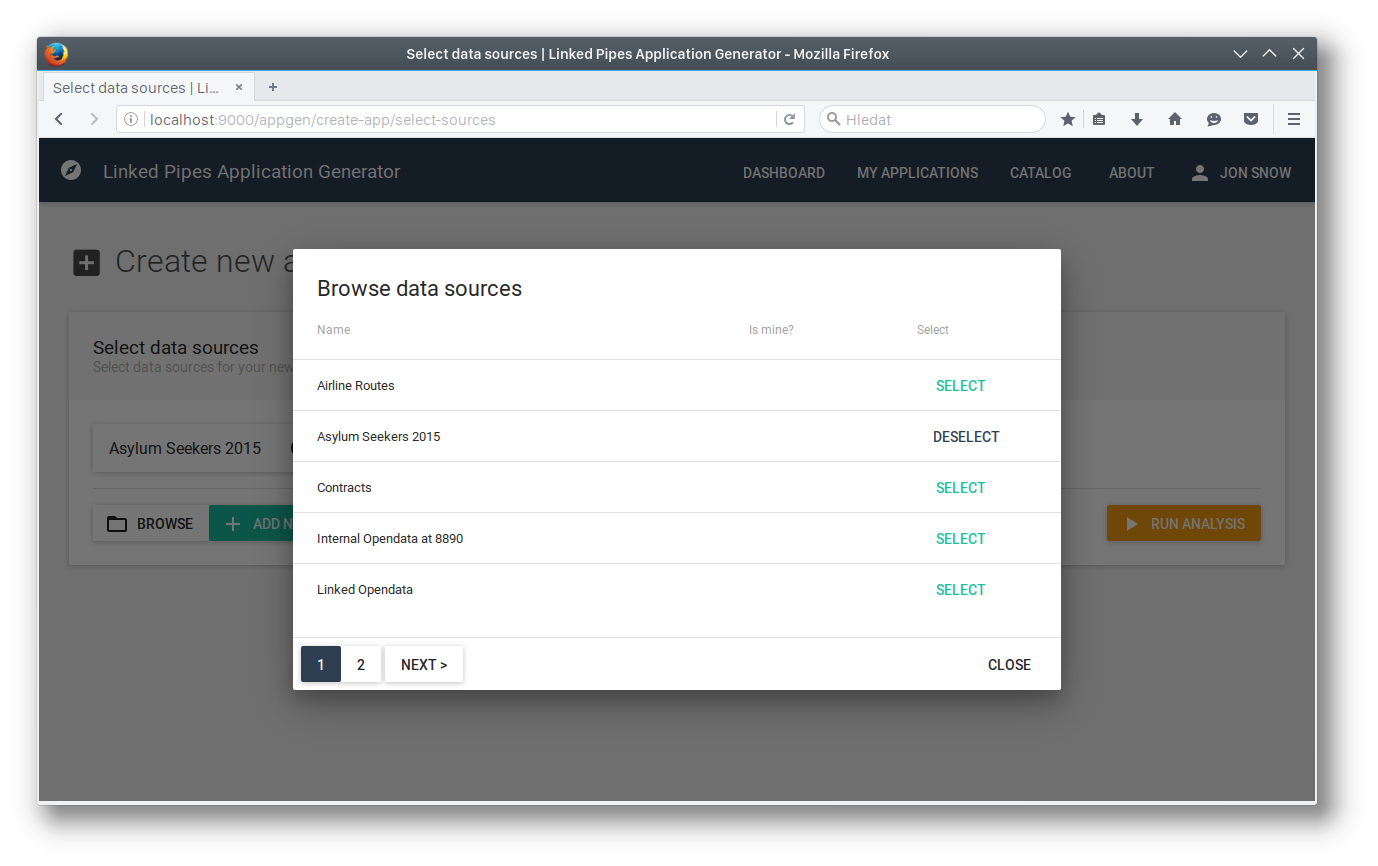
\includegraphics[width=145mm]{img/05_scenario_01_browse_data_sources.png}
	\caption{Use case scenario: Data source browser. The journalist selects the Asylum Seekers 2015 data set.}
	\label{fig:scenario-01-browse-data-sources}
\end{figure}

\begin{figure}
	\centering
	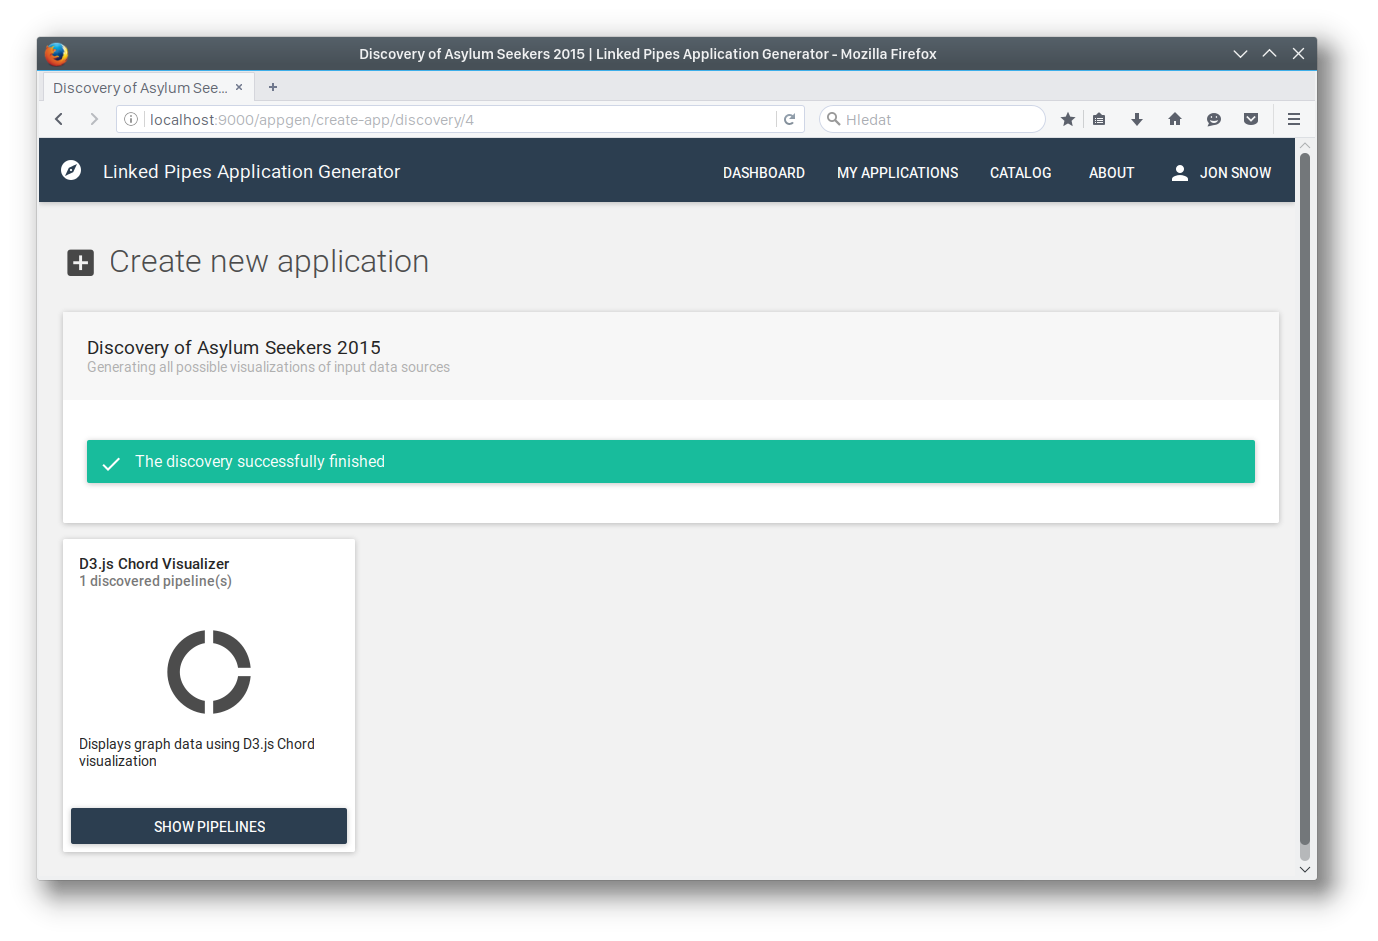
\includegraphics[width=145mm]{img/05_scenario_02_discovery_result.png}
	\caption{Use case scenario: Discovery result. The journalist can see that the Asylum Seekers 2015 data set can be visualized only using the D3.js Chord Visualizer. He runs the one discovered LDVM \emph{pipeline} that ends with this particular LDVM \emph{visualizer component}.}
	\label{fig:scenario-02-discovery-result}
\end{figure}

\begin{figure}
	\centering
	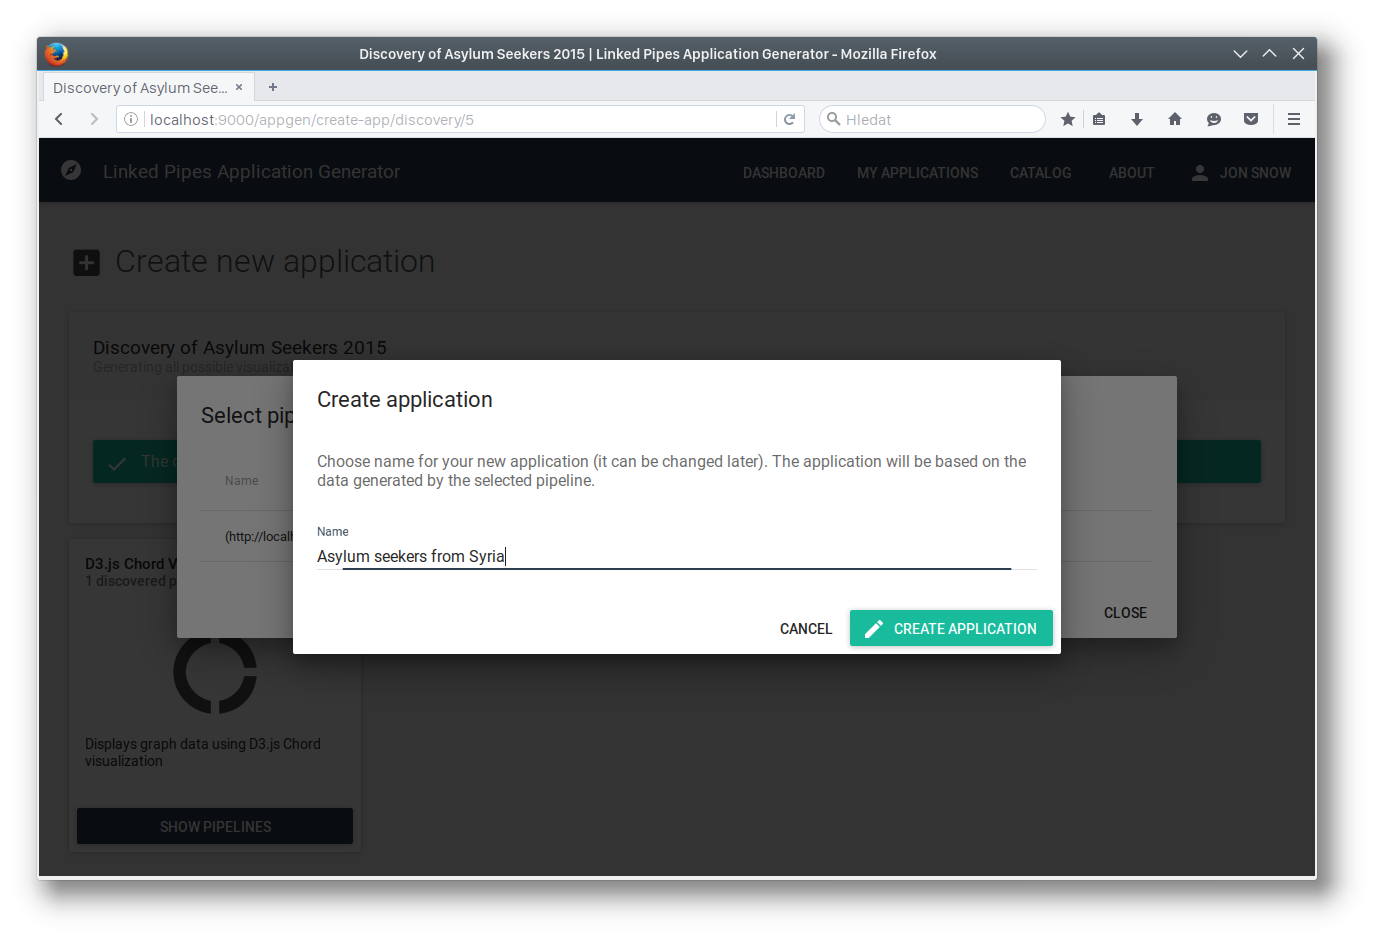
\includegraphics[width=145mm]{img/05_scenario_03_create_application.png}
	\caption{Use case scenario: Create application dialog. When the \emph{pipeline evaluation} is done, the user can proceed by creating an application.}
	\label{fig:scenario-03-create-application}
\end{figure}

\begin{figure}
	\centering
	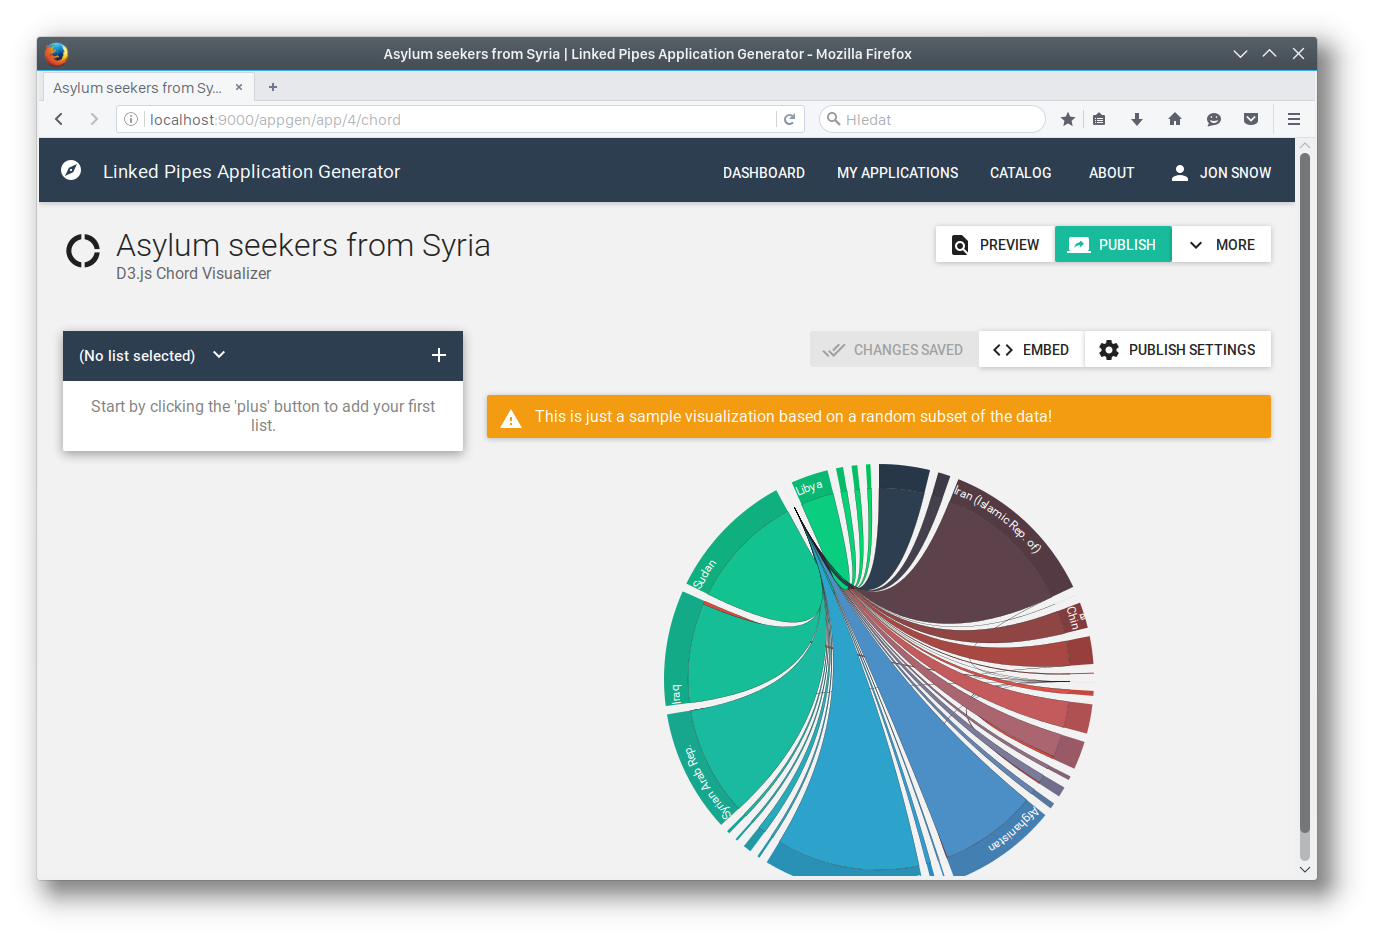
\includegraphics[width=145mm]{img/05_scenario_04_graph_sample.png}
	\caption{Use case scenario: Configurator of D3.js Chord Visualizer. Immediately after the application is created, the journalist is presented with a random sample visualization of the data.}
	\label{fig:scenario-04-graph-sample}
\end{figure}

\begin{figure}
	\centering
	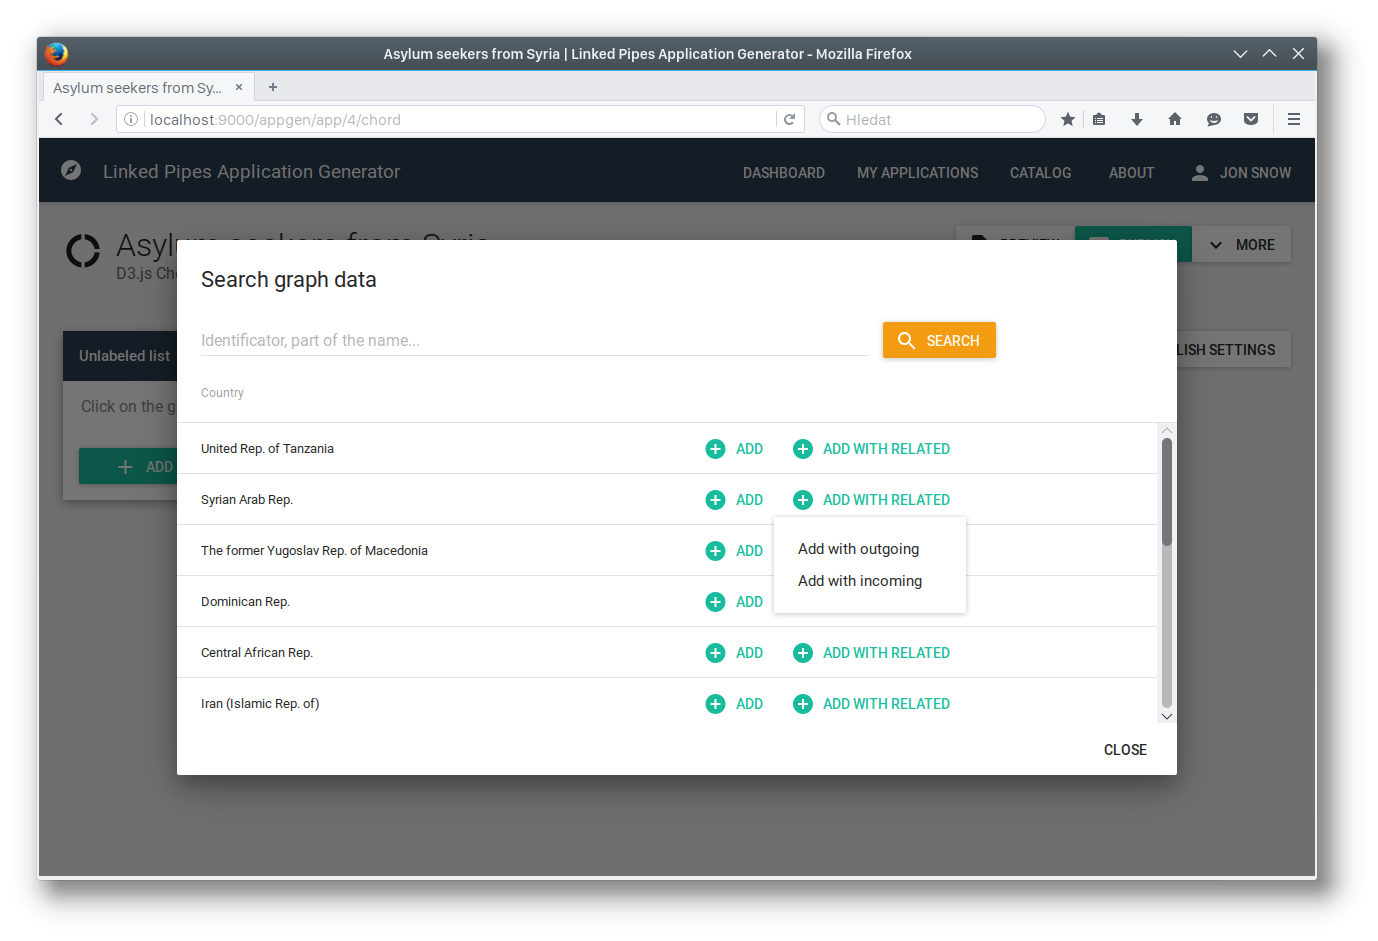
\includegraphics[width=145mm]{img/05_scenario_05_search_graph}
	\caption{Use case scenario: Search dialog. The journalist wants to create a visualization of asylum seekers coming from Syria. He uses the search feature to find Syria in the data set and adds it together with all target countries to the visualization \emph{list}.}
	\label{fig:scenario-05-search-graph}
\end{figure}

\begin{figure}
	\centering
	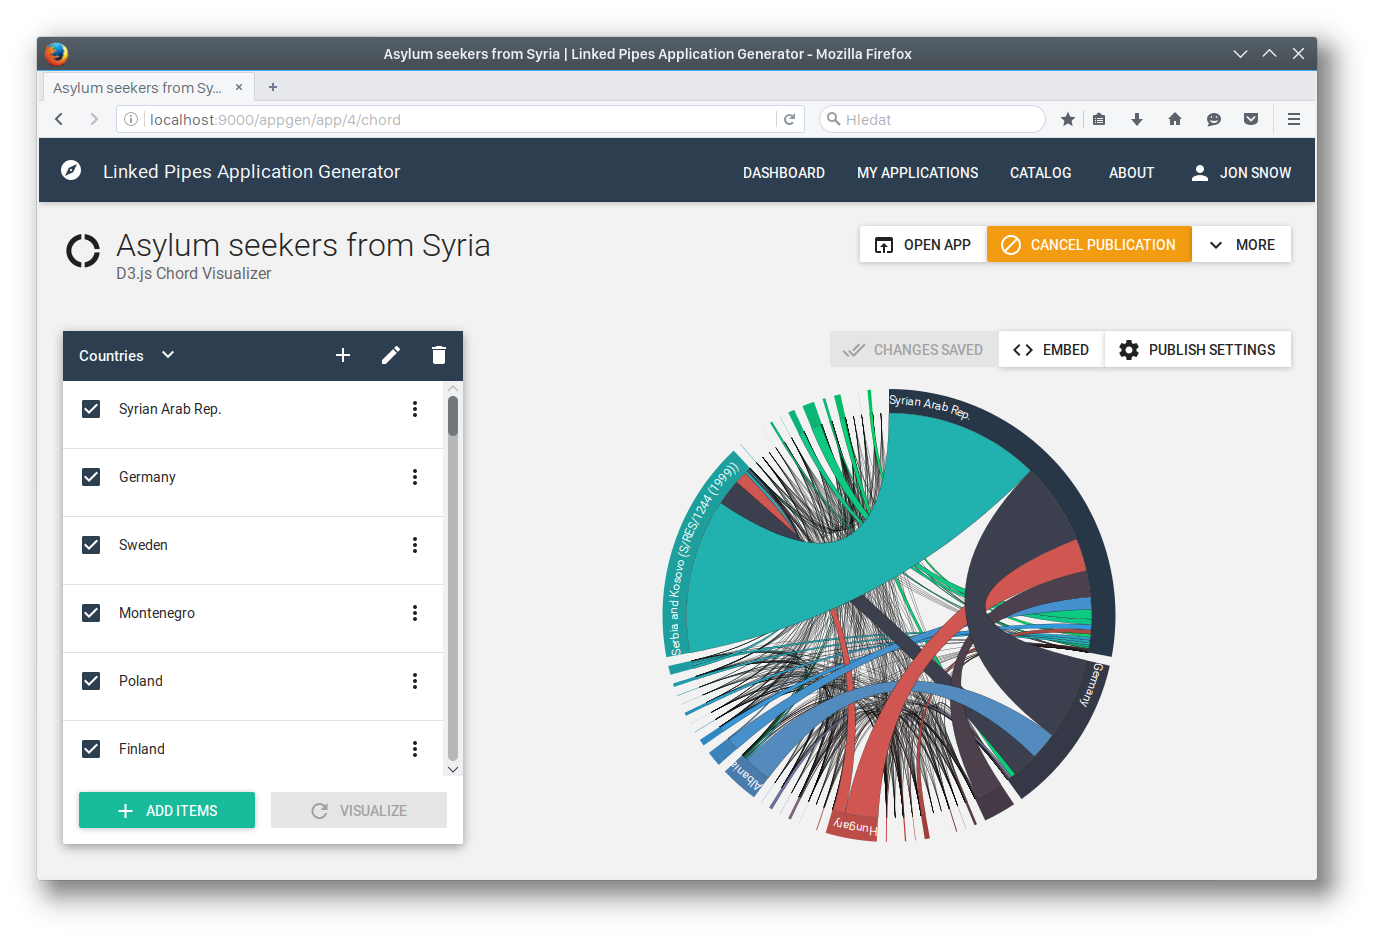
\includegraphics[width=145mm]{img/05_scenario_06_ready_application}
	\caption{Use case scenario: Visualization of selected countries. The journalist is now presented with the chord diagram of the countries he added into the \emph{list}.}
	\label{fig:scenario-06-ready application}
\end{figure}

\begin{figure}
	\centering
	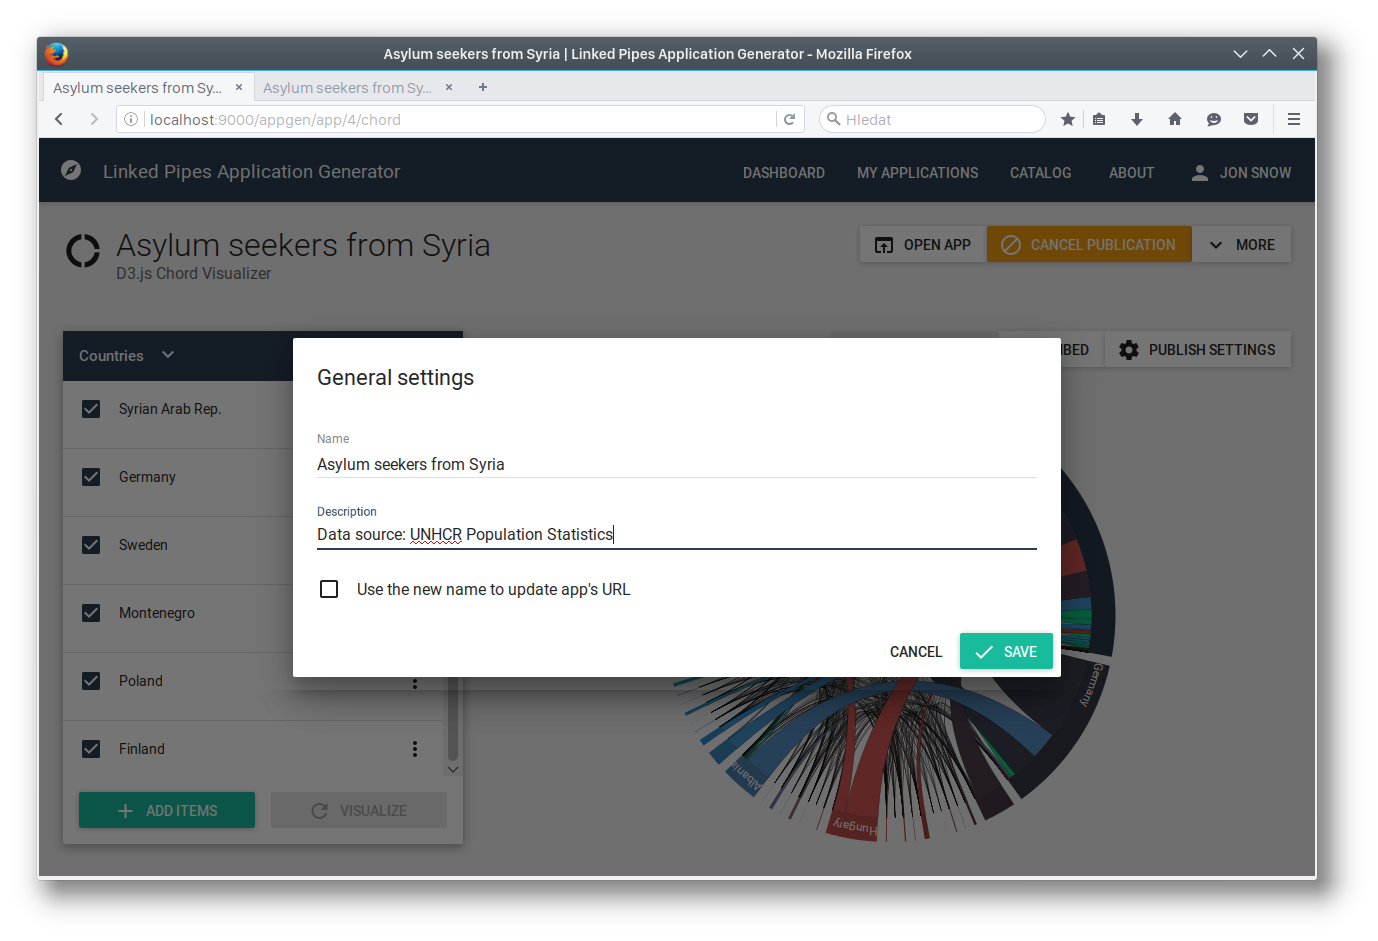
\includegraphics[width=145mm]{img/05_scenario_07_general_settings}
	\caption{Use case scenario: General application settings. The journalist can also provide the application description (in this case he uses it to explicitly mention the source of the data).}
	\label{fig:scenario-07-general-settings}
\end{figure}

\begin{figure}
	\centering
	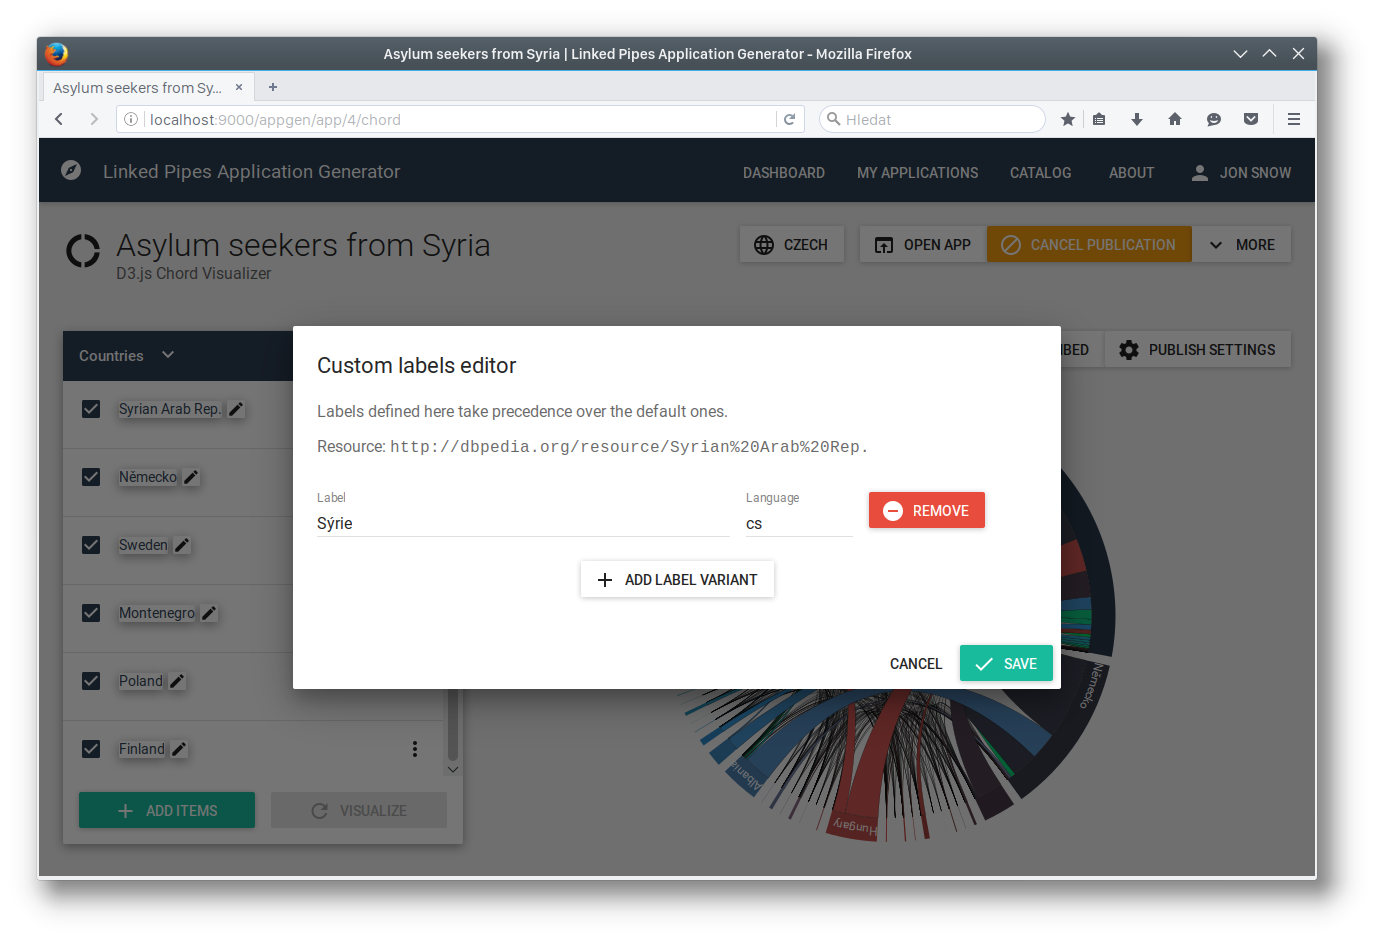
\includegraphics[width=145mm]{img/05_scenario_08_custom_label_editor}
	\caption{Use case scenario: Custom labels editor. The journalist is targeting Czech audience but the country names in the data set are in English. The configurator lets the journalist provide his own names that will override the default ones. }
	\label{fig:scenario-08-custom-label-editor}
\end{figure}

\begin{figure}
	\centering
	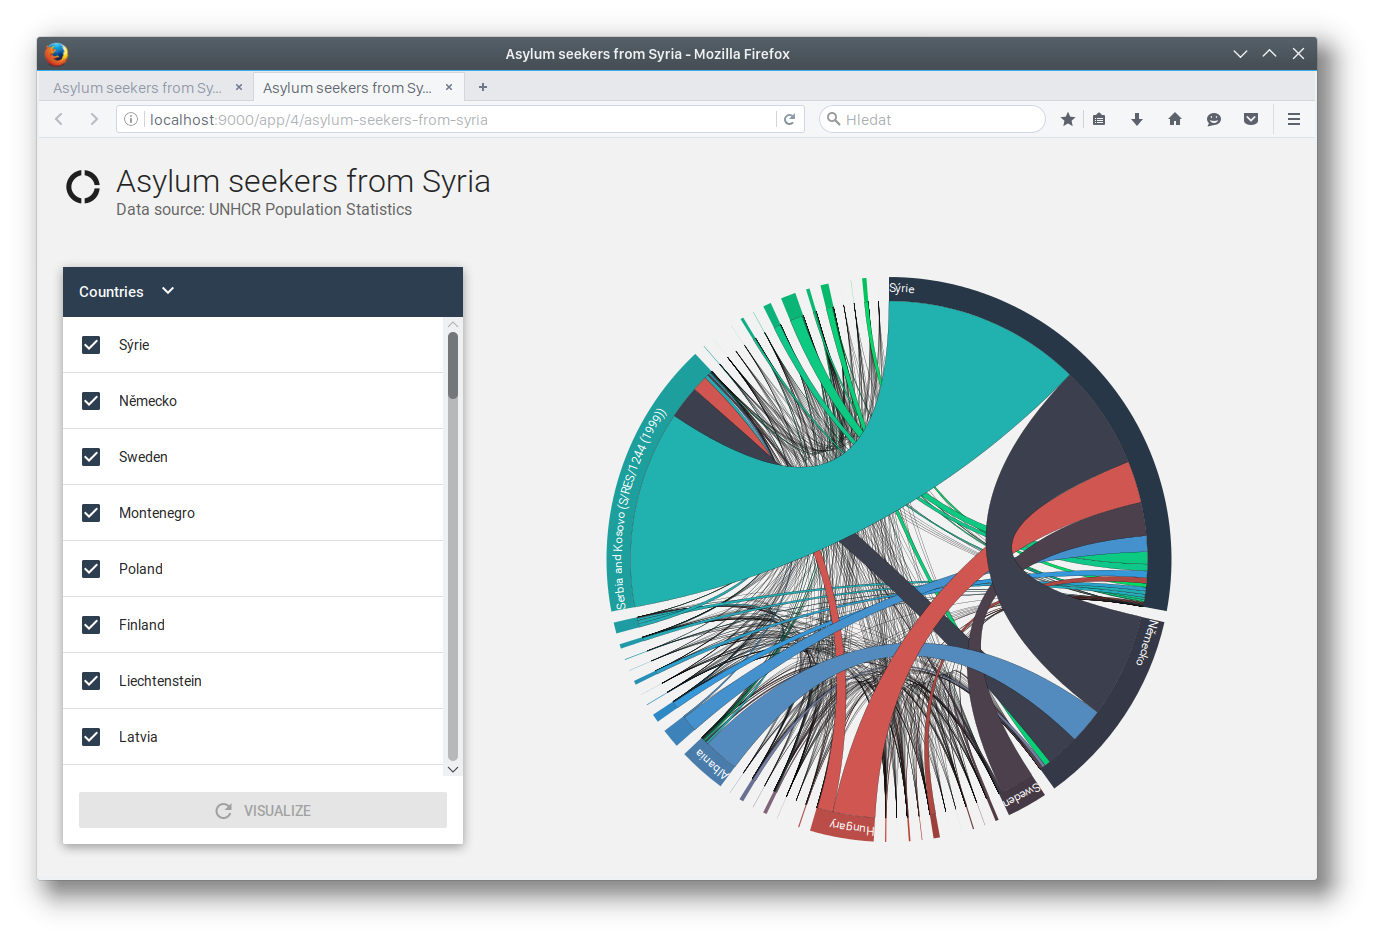
\includegraphics[width=145mm]{img/05_scenario_09_published_app}
	\caption{Use case scenario: Published application. This is what the journalist's readers will see when the application gets published. Using the menu on the side, the users can switch on/off individual countries in the chord diagram.}
    \label{fig:scenario-09-published-app}
\end{figure}

\begin{figure}
	\centering
	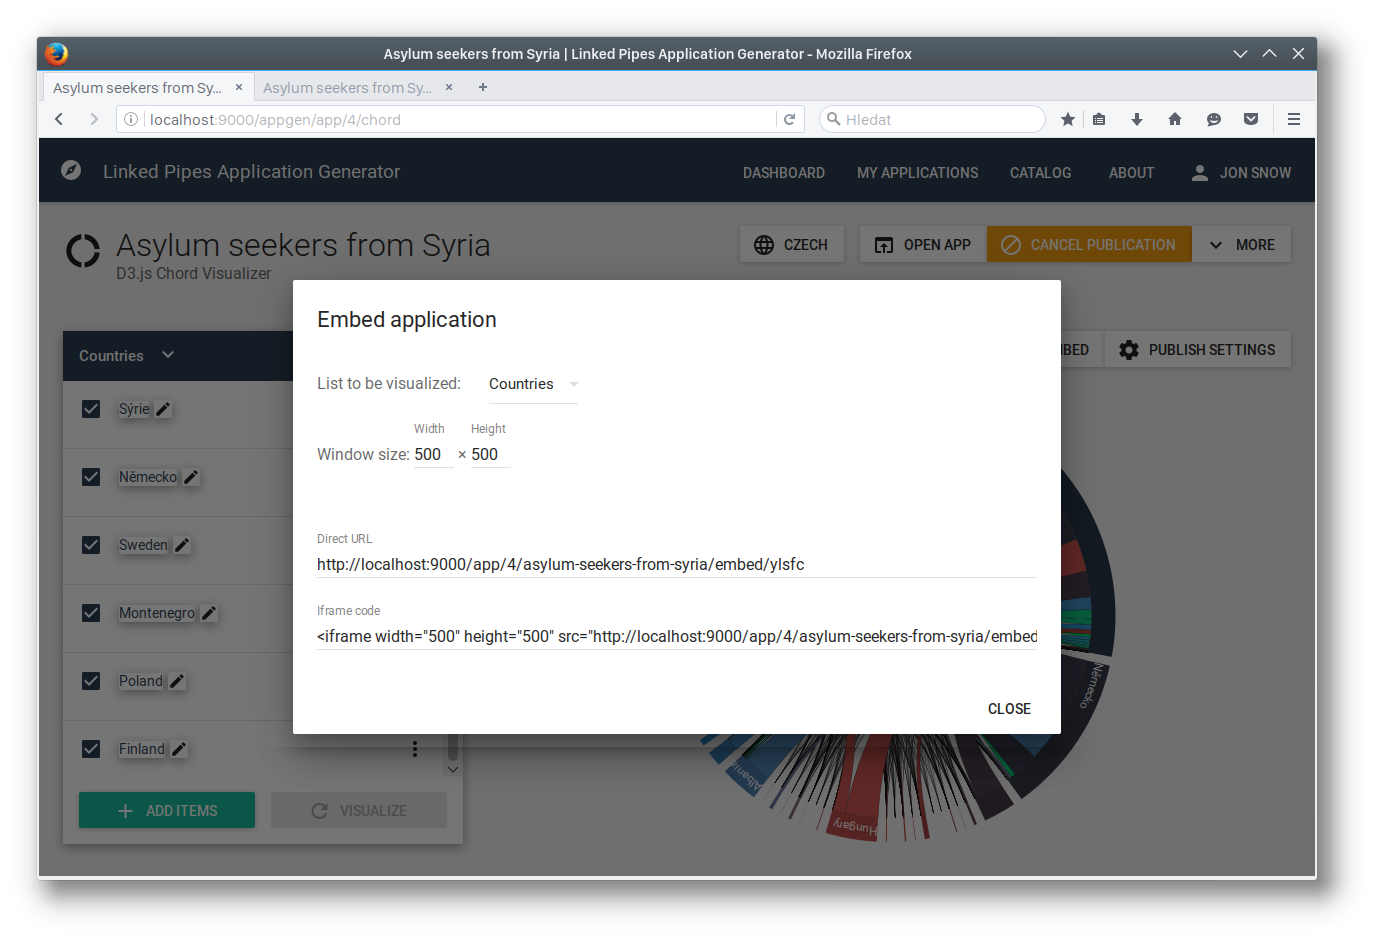
\includegraphics[width=145mm]{img/05_scenario_10_embed_application}
	\caption{Use case scenario: Embed application dialog. The journalist may decide to embed the chord diagram directly into his article.}
    \label{fig:scenario-10-embed-application}
\end{figure}

\begin{figure}
	\centering
	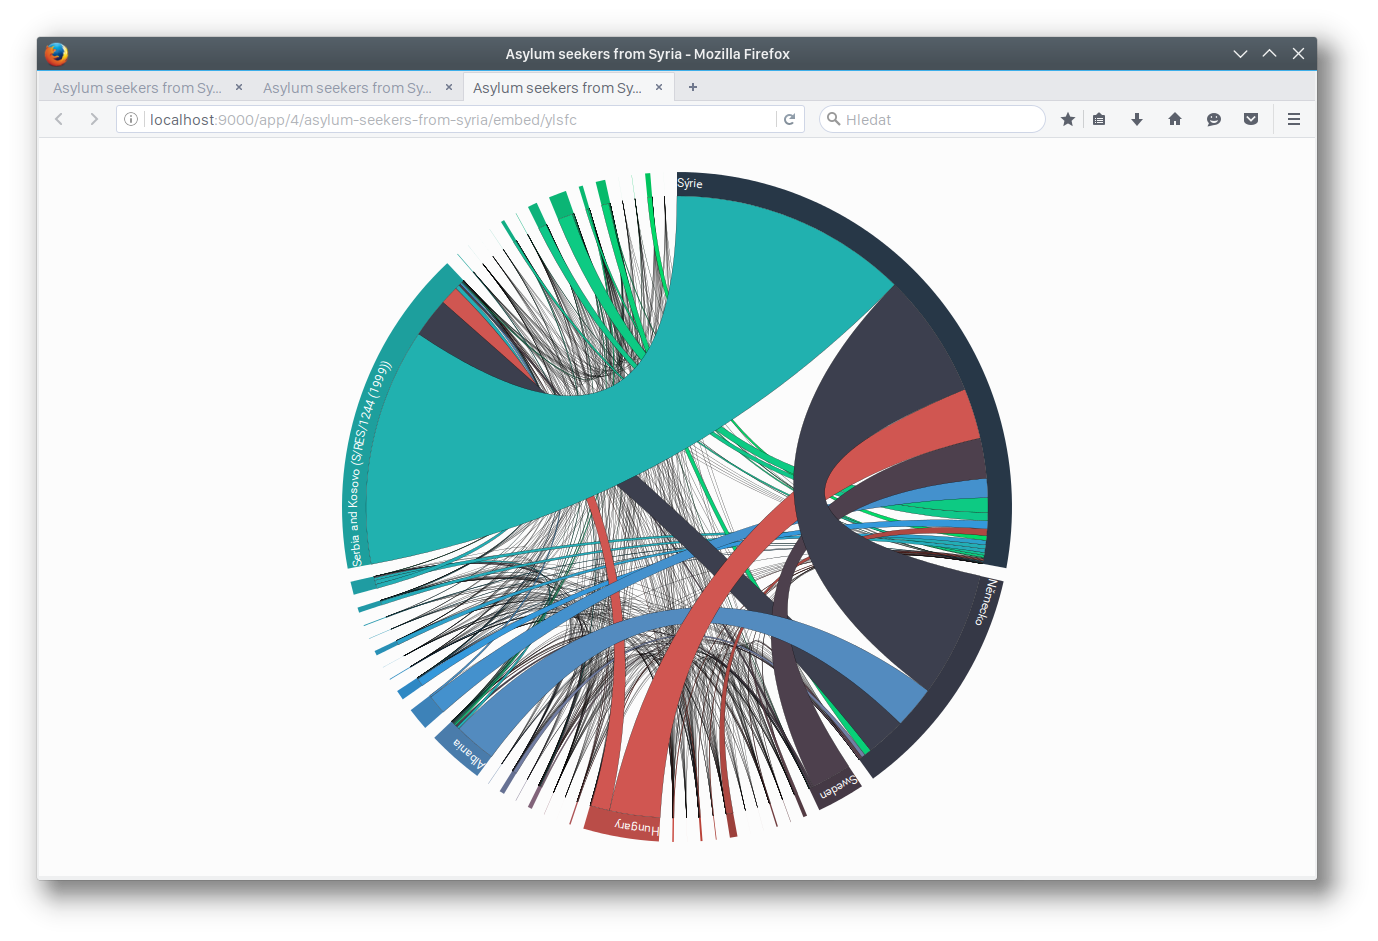
\includegraphics[width=145mm]{img/05_scenario_11_embedded_application}
	\caption{Use case scenario: Embedded application. In this form, stripped from all controls to the bare visualization, it is perfect for direct embedding into web pages.}
    \label{fig:scenario-11-embedded-application}
\end{figure}


\subsection{Users}

Everyone who wants to use our \emph{application generator} needs to create an account first. At this moment, a user can either create a standard local account protected by a password or he can log in with his Google account. No other providers are currently supported. As the user works with the \emph{application generator}, all his applications, data sources and discoveries are linked to his account and no one else can access it. E.g. an application can be configured only by its owner and before it is published, only the owner can view it.

One exception are \emph{administrator} accounts which work similarly to root users known from Unix systems. Such users can access and update any applications, data sources or discoveries in the system. The first user to register in our \emph{application generator} automatically becomes an administrator. The others have to be manually appointed (which is currently not possible through the user interface and has to be done by directly updating the database record).

\begin{figure}
	\centering
	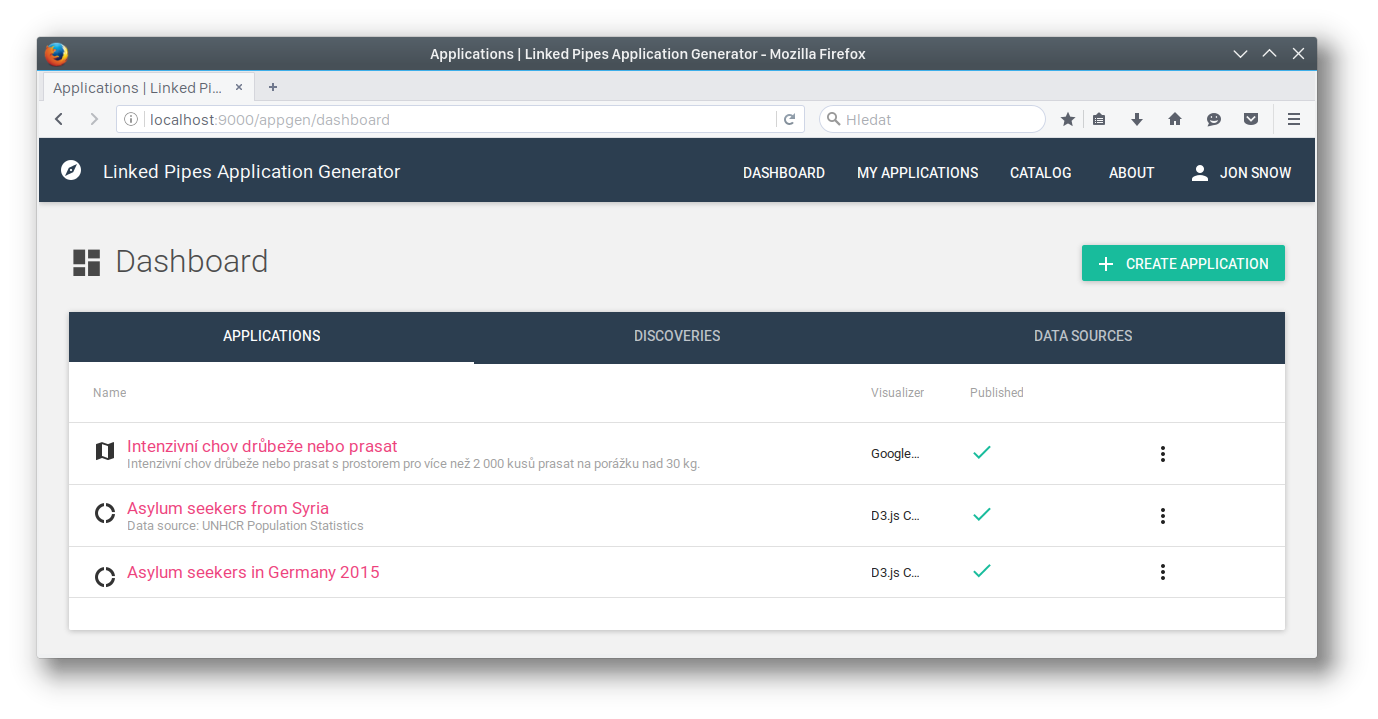
\includegraphics[width=145mm]{img/05_dashboard}
	\caption{User dashboard showing the overview of applications, discoveries and data sources}
    \label{fig:dashboard}
\end{figure}

\subsection{Data sources}

Our  approach to data sources is slightly different to LinkedPipes Visualization. In LinkedPipes Visualization, the user starts by providing the data source (may it be the SPARQL endpoint URL or a *.ttl file with serialized RDF data) and he has to do it every single time he wants to create a visualization. In our \emph{application generator}, we focused more on the possibility to re-use and share the data sets. So the user has to start by adding a data source to the generator, giving it a common name and only then he is allowed to select it for visualization. 

If we just have a new data set and want to get to a visualization quickly, the approach of LinkedPipes Visualization is faster. But once we want to re-use that data set, our approach wins over. 

That is not the only advantage. In our \emph{application generator}, we distinguish between public and private data sources. Private data sources are seen only by their owner (it should be mentioned that they are just hidden by the user interface, they are not actively protected from being used by other users). Public data sources, on the other hand, ale openly available for anyone and can be selected in the data source browser (Figure \ref{fig:scenario-01-browse-data-sources}). Any user can decide to make any of his data sources public. The idea is that one user (a data expert) might prepare the data set and another might use it to generate an application.

This approach introduces another level of abstraction. The user generating an application does not have to know what RDF or a SPARQL endpoint is, i.e, he is separated from the technical details. He can simply select the data source he is interested in from the browser and use it.

\subsection{Pipeline discovery}

The \emph{application generator} runs the underlying LDVM \emph{discovery} algorithm on the selected data sources. The \emph{discovery} returns all possible LDVM \emph{pipelines} that lead to a visualization, i.e., they end with a \emph{visualizer component}. Multiple \emph{pipelines} might use the same \emph{visualizer component} (they might use different \emph{analyzers} and \emph{visualizer transformers} along the way to get the input data compatible with this particular visualizer). Unfortunately, we are not able to give the user any detailed information about how the data produced by a \emph{pipeline} will look like. The only way to find out is to actually run the \emph{pipeline} and create an application from it. If the data do not make sense or are not what the user expects, he can try another one.

The user can watch the \emph{discovery} algorithm progress on a dedicated screen that shows the current \emph{discovery} status and also the list of \emph{pipelines} that have been discovered so far (Figure \ref{fig:scenario-02-discovery-result}). The \emph{pipelines} are grouped by \emph{visualizers}. As the algorithm may take some time, the user can leave the screen and come back later. It is accessible even after the \emph{discovery} algorithm finishes. The list of all discoveries can be found on the dashboard \ref{fig:dashboard}.

Note that not all \emph{visualizer} are supported by our \emph{application generator} (i.e., the corresponding \emph{plugin} is missing). For example, LinkedPipes Visualization contains a \emph{visualizer} for statistical data described using Data Cube Vocabulary \cite{datacube_vocabulary}. If the appropriate LDVM \emph{component} is registered in our \emph{application generator}, the \emph{discovery} algorithm will return \emph{pipelines} that use this \emph{component}. However, those will not be offered to the user.

\subsection{Application configuration}

The configuration phase is the core feature of the \emph{application generator} which differentiates it from the LinkedPipes Visualization. The application configuration involves both tasks that are common for all applications (e.g. publishing, deleting, updating description etc.) and that are \emph{visualizer} specific. As you can see on the Figure \ref{fig:configurator}, the \emph{configurator} interface follows this principle. It is divided into the common area and the area which is controlled by a particular \emph{visualizer} plugin (see Figure \ref{fig:google_maps_visualizer} of how a different \emph{visualizer} adapts to the universal configurator interface). 

\begin{figure}
	\centering
	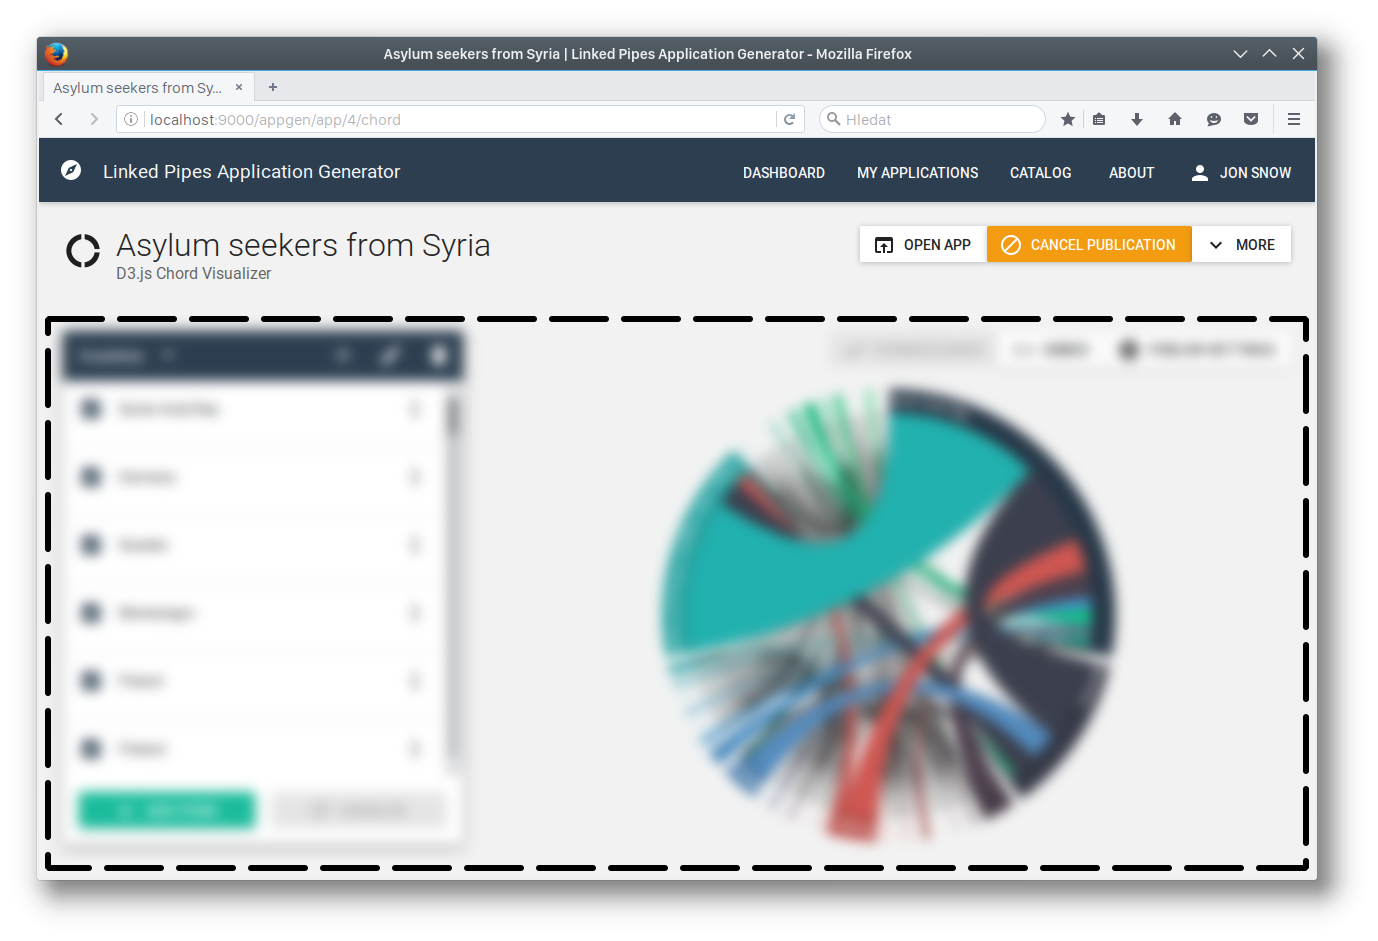
\includegraphics[width=145mm]{img/05_configurator.png}
	\caption{The configurator interface. The blurred out part is controlled by the current visualizer whereas the rest is identical for all visualizers. It contains the common functionality (e.g. the "More" button in the upper right corner shows a menu allowing the user to delete the application or change the application name and description).}
    \label{fig:configurator}
\end{figure}

\begin{figure}
	\centering
	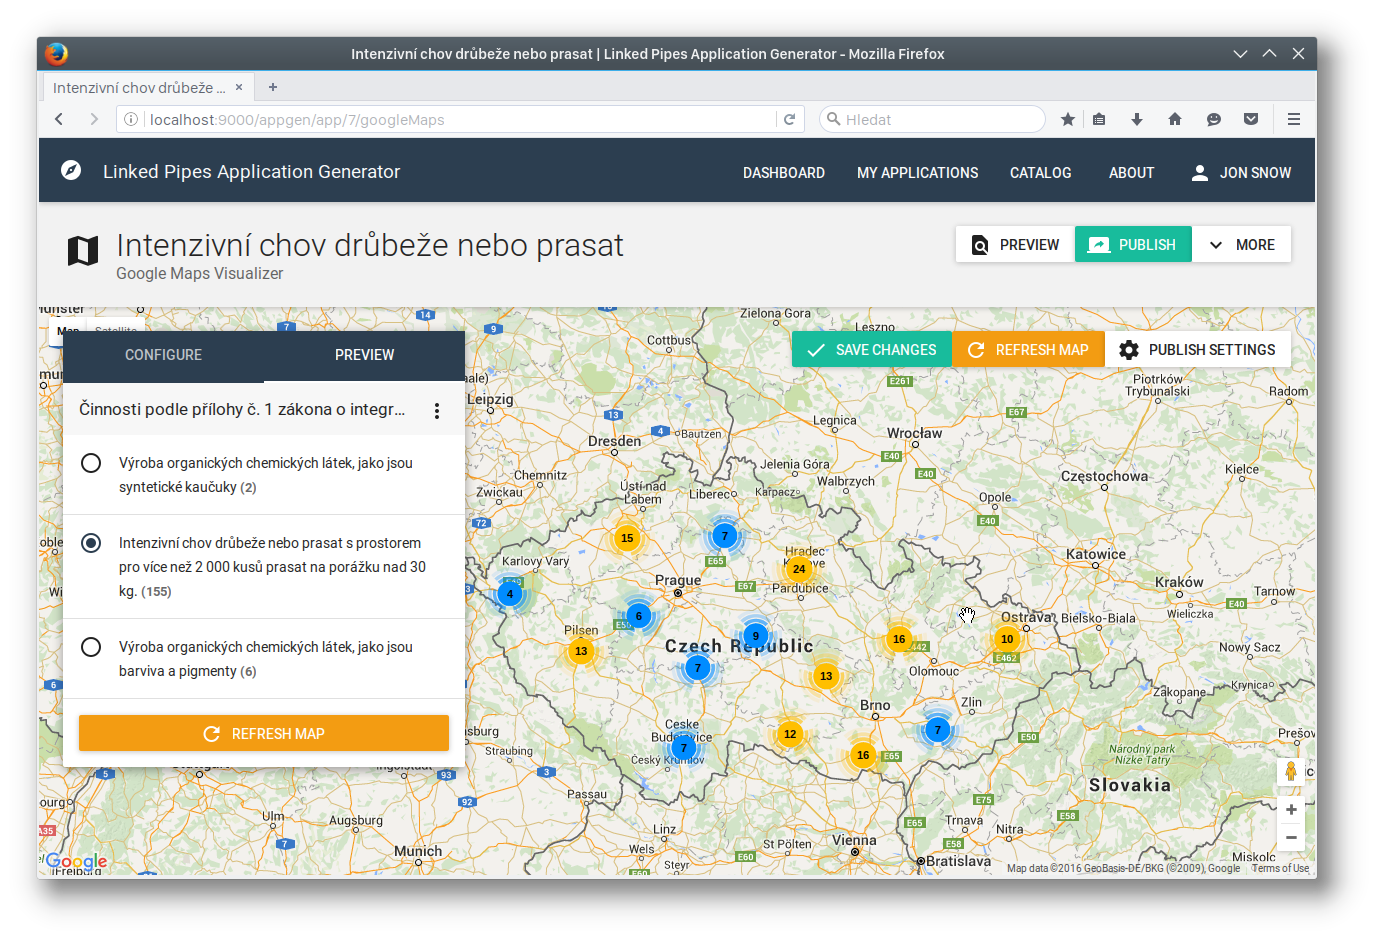
\includegraphics[width=145mm]{img/05_google_maps_visualizer.png}
	\caption{The configurator interface of the Google Maps Visualizer.}
    \label{fig:google_maps_visualizer}
\end{figure}

\subsection{Publishing applications}

When the user is happy with how the application looks, he can publish it by hitting the green "Publish button" (as seen for example on the Figure \ref{fig:scenario-04-graph-sample} in the upper right corner). The application then becomes accessible on a public URL which is generated from the application ID (internal numeric identificator) and its name. The \emph{application generator} at this moment does not offer any fine grained control of who gets to access the application. It is either public or not. Once it is published, it also becomes part of the public application catalog (Figure \ref{fig:catalog}).

\begin{figure}
	\centering
	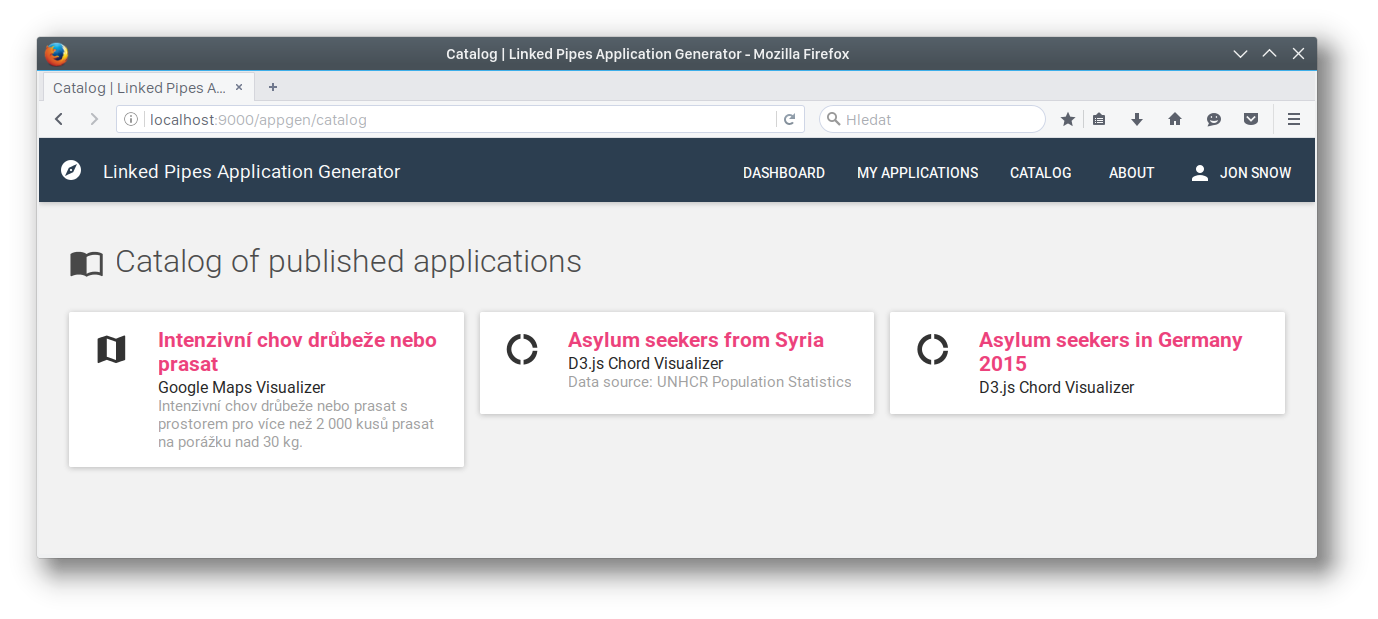
\includegraphics[width=145mm]{img/05_catalog}
	\caption{Catalog of published applications.}
    \label{fig:catalog}
\end{figure}

Some \emph{visualizers} offer the option to publish the application in an embed mode. That means that the application's interface is adapted so that it can be inserted for example into an external online article. The interface is usually significantly reduced and stripped from unimportant  control elements. This functionality is not considered common for all \emph{visualizers}  as each \emph{visualizer} can approach it differently. For example, the D3.js Chord Visualizer we used in this section allows the user to create multiple chord diagrams within a single application. Each of these diagrams can be exported separately in the embed mode (a unique URL is generated for each diagram under which the diagram is accessible). See Figure \ref{fig:scenario-10-embed-application}. Clearly, this functionality is specific for D3.js Chord Visualizer.

\section{General architecture}

We decided that we build our \emph{application generator} on top of LinkedPipes Visualization (Section \ref{sec:system_proposal:integration}). We already described the architecture of this tool (Section \ref{sec:linkedpipes:architecture} and especially Figure \ref{fig:linked-pipes-visualization-architecture}). We will now explain how we integrated the \emph{application generator} into LinkedPipes Visualization. You will get the overall idea by referring to Figure \ref{fig:application-generator-architecture}.

\begin{figure}
	\centering
	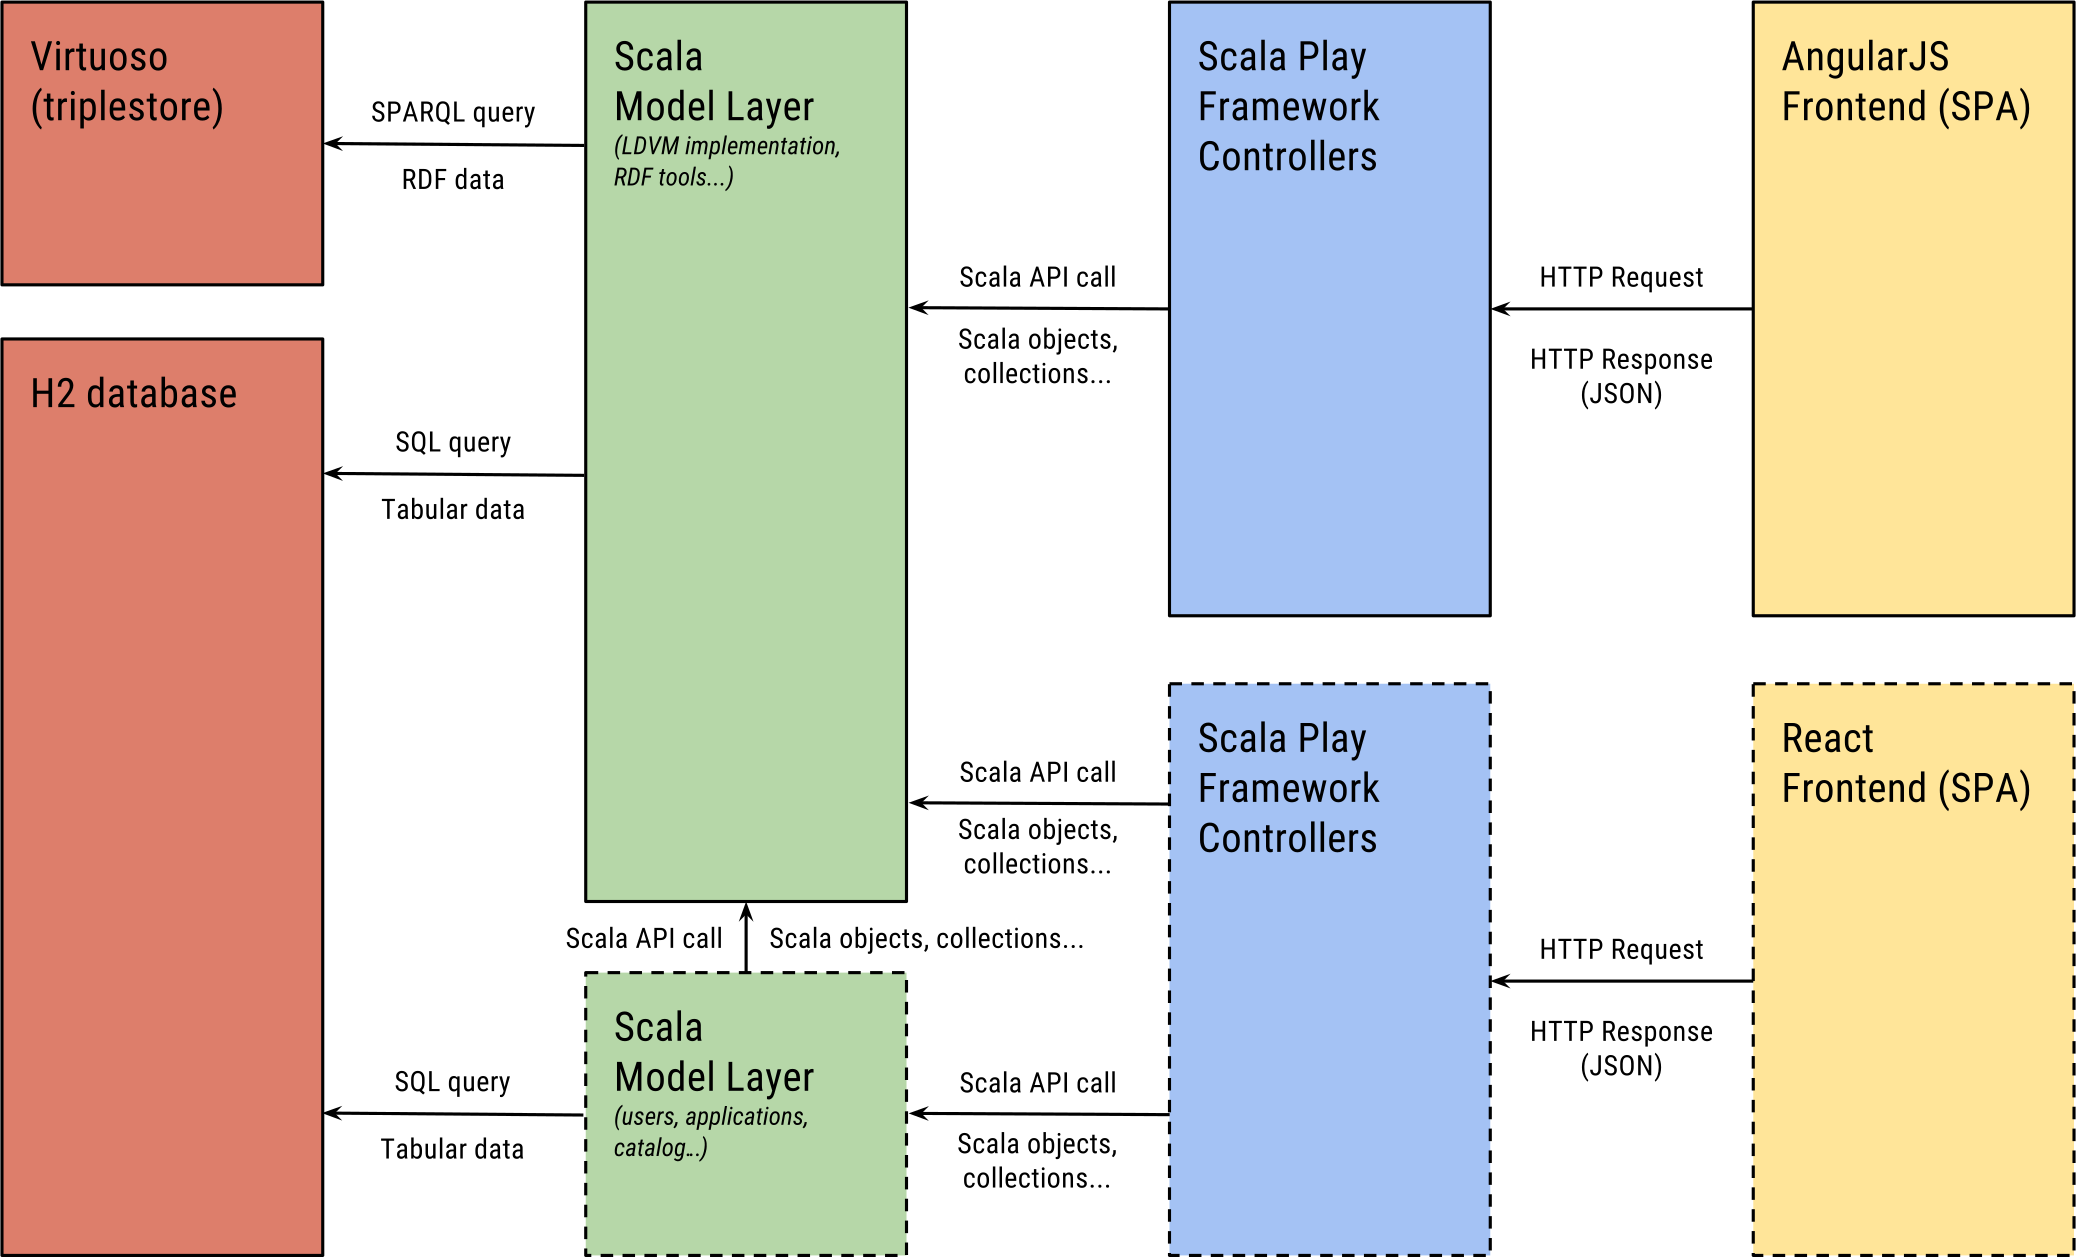
\includegraphics[width=140mm]{img/05_application_generator_architecture.png}
	\caption{Application Generator Architecture. Blocks with solid borders are part of the original LinkedPipes Visualization, blocks with dashed borders are newly implemented parts of the \emph{application generator}.} 
	\label{fig:application-generator-architecture}
\end{figure}

The \emph{application generator} is part of the original LinkedPipes Visualization code base. We made this decision after consulting the authors of LinkedPipes Visualization. From the software architectonic perspective, it is probably not the cleanest approach, but it significantly sped up our work. The original code base contained many solutions and APIs that we could immediately use (for example the LDVM implementation API, various RDF tools etc.). Nevertheless, even though both tools live in the same code base, we made sure to keep them as separated as possible (Figure \ref{fig:application-generator-architecture} shows that clearly). So if we decided in the future to separate both tools or for example replace the underlying LDVM implementation, it should not be impossible.

An important consequence of this unification is that the LDVM implementation instance is shared among the \emph{application generator} and LinkedPipes Visualization. That means that they both use the same set of registered LDVM \emph{components}. We benefited from this as well to an extent. Due to the lack of time, we did not manage to implement all user interfaces for our generator. For example, new LDVM \emph{components} are registered to the \emph{generator} through the LinkedPipes Visualization user interface.

\subsection{Frontend}

The \emph{application generator} frontend is completely new and independent on the original frontend. The original frontend already contained some work that we could at first glance use (e.g. existing \emph{visualizer} plugins). Unfortunately, couple of problems prevented us from doing so. Firstly, the AngularJS frontend was created just to showcase the capabilities of the underlying LVDM implementation. For this reason, its code was in a rather poor state with no documentation. Clearly, it would take us lots of time to get familiar with it. Secondly, this code was not written with certain features (like for example user support) in mind. Thirdly, our \emph{visualizers} (with the separated \emph{configurator} and \emph{application} interfaces) work very differently compared to the \emph{visualizers} of LinkedPipes Visualization. Having these three reasons in mind, we came to the conclusion that we would have to rewrite a major portion of the original code anyway and therefore we decided to start from the scratch. We also decided to go with a different development stack (we replaced AngularJS with React and related tools) which we believed would fit our needs better. 

As a result, there are two existing user interfaces that live within the same application next to each other. The original LinkedPipes Visualization interface is accessible from the home page (the \texttt{/} URL). Our \emph{application generator} can be found at \texttt{/appgen} and individual published applications live at \emph{/app}.

\subsection{Controllers}

The vast majority of controllers in both LinkedPipes Visualization and the \emph{application generator} handle the asynchronous HTTP requests coming from the frontend (the only exception are the controllers handling the initialization of the SPAs). The role of a controller in this typical case is just to translate the HTTP request into an API call to the \emph{Model} layer and send the response back. All controllers together define a public remote API interface.

Even though we could re-use some of the methods available from the LinkedPipes Visualization controllers (e.g. those for controlling the \emph{discovery} algorithm), we decided not to do that to avoid hidden dependencies between the frontend and the backend. Dependencies within the Scala code base (for example between the \emph{Controller} layer and the \emph{Model} layer) are easy the discover. If they break, the code will not compile. That is not true for the remote API. Therefore the \emph{application generator} frontend strictly uses only those remote API methods that are handled by the \emph{application generator} controllers. They all exist in a standalone \texttt{controllers.appgen} Scala package.

\subsection{Model}

The \emph{Model} layer consists of various repositories and services that handle the business logic. The repositories and services that specifically handle the \emph{application generator} business logic (e.g. application management, users etc) can all be found in the \texttt{model.appgen} package.

The \emph{Model} layer among other things contains tools for working with RDF data, e.g. services converting RDF data in various vocabularies into Scala objects. While we were developing our \emph{visualizers}, we needed to add support for some new vocabularies to the code base. This is the only case when our code significantly overlaps with the original LinkedPipes Visualization code. However, this code is not specific to our \emph{application generator}, it actually extends the functionality of LinkedPipes Visualization.

Figure \ref{fig:application-generator-architecture} might suggest that our extension of the \emph{Model} layer directly communicates with the H2 database. Strictly speaking, that is not true because we are utilizing some low level services to access the database and those services could still be considered part of the \emph{Model} layer.

What is important is that all \emph{application generator} related Scala code exists in those two packages (\texttt{controllers.appgen} and \texttt{model.appgen}). Also the frontend strictly communicates only  with our controllers. Therefore it is easy to draw the line where LinkedPipes Visualization ends and our \emph{application generator} begins. Dependencies between our code and the original code base are shown on Figure \ref{fig:application-generator-architecture} and are always a matter of Scala code. The dependencies are in a form of utilizing the internal API of LinkedPipes Visualization. In rare cases, we re-use some low-level utilities from the original code base.

\section{Scala backend utilities}

% Simple, following the architecture of LinkedPipes Visualization

% Each visualizer has its own controller (explain why)

% Extending inner structures (user id). The original ones are not being deleted

% Framework: Cache? Controllers?

% RDF vocabularies


\section{Frontend development stack}

\subsection{ES6 and Babel compiler}

\subsection{React}

\subsection{Redux}

\subsection{Reslect}

\subsection{React-router}

% Explain why routing is important (back button)

\subsection{Immutable.js}


\section{Frontend framework architecture (???)}

\subsection{JavaScript bundles}

% webpack endpoints / bundles -> /appgen

\subsection{Code structure}

% assets folder
% explain where can be found what

\subsection{Modules}

% prefixing
% problem with automatic name extraction from the folder name
% module structure
% routes

\subsection{Ducks}

\section{Process of creating a new application from the code perspective}

Describing the inner mechanics for the whole \emph{application generator} would take us too long and this description is not that important for the reader anyway. We will just walk through the use case scenario again (Subsection \ref{sec:implementation:use-case-scenario}) and describe what is going on under the hood. Among other things, this should help the reader to better understand how integration of new \emph{visualizers} into the \emph{application generator} works.

% TODO

\section{Integrating a new visualizer}

Now that the reader is equipped with all the necessary knowledge, we will walk him through the process of creating a brand new \emph{visualizer} to demonstrate the abilities of our framework. The \emph{visualizer} will be visualizing a graph (as understood in the graph theory) represented with the RGML vocabulary (which makes it very similar to the D3.js Chord Visualizer that will be properly described later, including the vocabulary). The purpose of this section is merely to get the reader familiar with the basic integration steps. The presented \emph{visualizer} will simply display number of vertices and edges of the graph and let the user configure the graph label.

\subsection{LDVM component}

We start be defining the LDVM \emph{visualizer component} using the \texttt{ldvm} vocabulary. As the whole definition would be pretty long, we will walk through it statement by statement and provide necessary explanations. Let us start with couple of prefixes for vocabularies that we are going to use.

\scriptsize
\begin{verbatim}
@prefix rdfs:  <http://www.w3.org/2000/01/rdf-schema#> .
@prefix dcterms: <http://purl.org/dc/terms/> .
@prefix ldvm: <http://linked.opendata.cz/ontology/ldvm/> .
\end{verbatim}
\normalsize

Now let us add prefixes identifying the new \emph{visualizer}. The \texttt{v} stands for "visualizer", the \texttt{r} stands for "resource" and \texttt{graph} is the short name that we will be using for our \emph{visualizer}.

\scriptsize
\begin{verbatim}
@prefix v-graph: <http://linked.opendata.cz/ontology/ldvm/visualizer/graph/> .
@prefix v-graph-r: <http://linked.opendata.cz/resource/ldvm/visualizer/graph/> .
\end{verbatim}
\normalsize

What follows now is the definition of the main RDF resource representing our \emph{visualizer} that binds everything together.

\scriptsize
\begin{verbatim}
v-graph-r:GraphVisualizerTemplate a ldvm:VisualizerTemplate ;
    rdfs:label "Graph Visualizer"@en;
    rdfs:comment "Visualizes graph data"@en;
    ldvm:componentConfigurationTemplate v-graph-r:Configuration ;
    ldvm:inputTemplate v-graph-r:Input ;
    ldvm:feature v-graph-r:GraphFeature ;
    .
\end{verbatim}
\normalsize

Do not be confused by the word \texttt{Template}. In LDVM, even the \emph{pipelines} themselves are represented in RDF. Each \emph{pipeline} consists of \emph{component instances} that are instantiated from \emph{component templates} just like this one.

As you can see, this \emph{component} has a \emph{configuration}, one \emph{input} and one \emph{feature}. There is nothing important now about the \emph{configuration} and also the \emph{input} is pretty straightforward, so we will just drop here the definitions.

\scriptsize
\begin{verbatim}
v-graph:GraphVisualizerConfiguration a rdfs:Class ;
    rdfs:label "Graph Visualizer Configuration"@en;
    rdfs:subClassOf ldvm:ComponentConfiguration ;
    .
  
v-graph-r:Configuration a v-graph:GraphVisualizerConfiguration ;
    dcterms:title "Default Configuration" ;
    .

v-graph-r:Input a ldvm:InputDataPortTemplate ;
    dcterms:title "Graph data described using RGML vocabulary" ;
    .
\end{verbatim}
\normalsize

Let us now define the \texttt{GraphFeature}.

\scriptsize
\begin{verbatim}
v-graph-r:GraphFeature a ldvm:MandatoryFeature ;
    dcterms:title "The actual graph data, i. e. nodes and edges" ;
    ldvm:descriptor v-graph-r:GraphDescriptor ;
    .
\end{verbatim}
\normalsize

As you can see, this \emph{feature} is \emph{mandatory} which means that the input data must meet the requirements defined by the \emph{feature descriptor}. So let us have a look at it.

\scriptsize
\begin{verbatim}
v-graph-r:GraphDescriptor a ldvm:Descriptor ;
    dcterms:title "Graph presence check" ;
    ldvm:query """
        PREFIX rdf: <http://www.w3.org/1999/02/22-rdf-syntax-ns#>
        PREFIX rgml: <http://purl.org/puninj/2001/05/rgml-schema#>

        ASK {
            ?graph rdf:type rgml:Graph ;
                rgml:directed ?directed .

            ?edge rdf:type rgml:Edge ;
                rgml:source ?source ;
                rgml:target ?target ;
                rgml:weight ?weight .

            ?source rdf:type rgml:Node .
            ?target rdf:type rgml:Node .
        }
    """ ;
    ldvm:appliesTo v-graph-r:Input ;
    .
\end{verbatim}
\normalsize

The SPARQL query contained in the \emph{descriptor} is looking for a graph instance and at least one edge between two vertices. This requirement is applied on the input that we have defined before. If we put this all together we get that \textit{the \emph{mandatory feature} requires the data flowing through the only \emph{component input} to contain a non-empty graph}. So we have just specified how the RDF data coming to our \emph{visualizer} should look like.

What we have to do now is put all these lines together into a single *.ttl file (we have been using the Turtle syntax) and upload it to the \emph{application generator}. Unfortunately, the user interface for this task is not yet available inside the \emph{application generator} and we need to use LinkedPipes Visualization interface for it. So go to the homepage, open the left side menu, click \textbf{Components} and then the green \textbf{Add} button. It should get you to a screen that you can see on Figure \ref{fig:upload_component_definition}. Use the form to upload the definition.

\begin{figure}
	\centering
	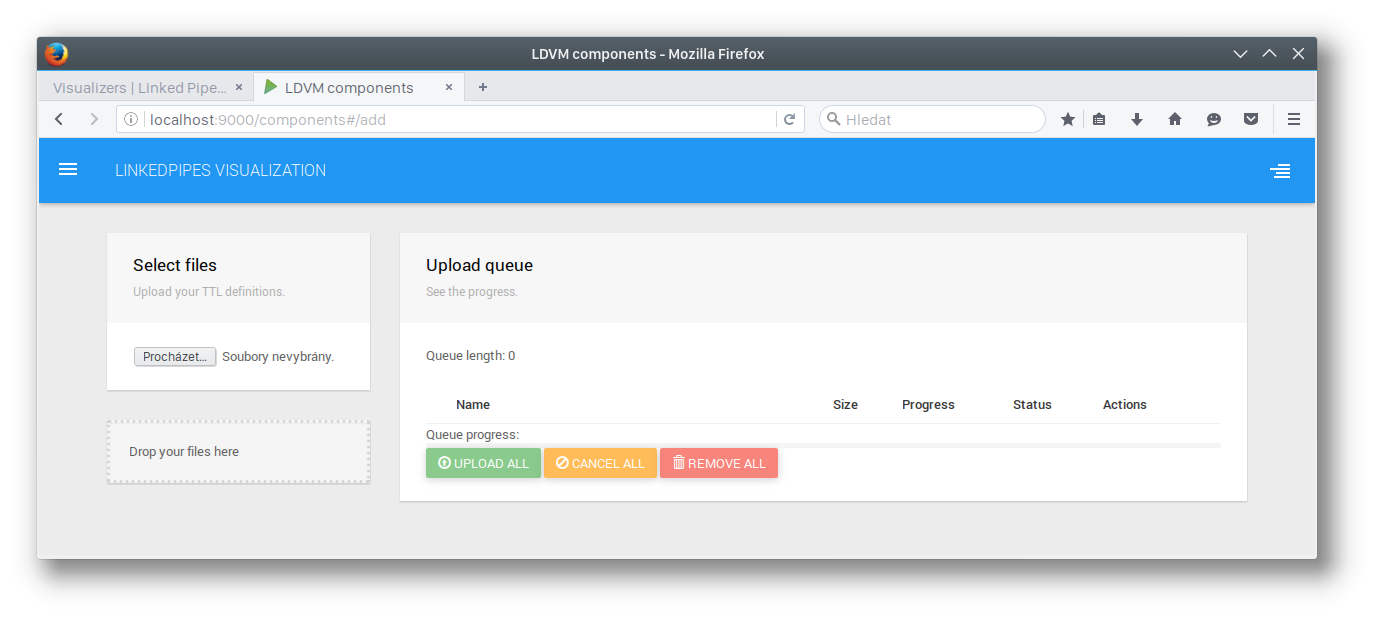
\includegraphics[width=145mm]{img/05_upload_component_definition.png}
	\caption{LinkedPipes Visualization: Upload component definition}
    \label{fig:upload_component_definition}
\end{figure}

Once this is done, the \emph{discovery} algorithm is able to utilize this new \emph{visualizer component} when discovering pipelines. If you now ran the \emph{discovery} inside LinkedPipes Visualization on a data set containing some graph data, it should find a \emph{pipeline} ending with this \emph{visualizer component}. Now we need to implement the corresponding \emph{visualizer plugin} for our \emph{application generator}.

\subsection{Frontend module}

As the first thing, we need to choose a unique short name for our \emph{visualizer}. When creating the RDF definition, we used the name \texttt{graph} as a RDF prefix. We will stick to this name.

A \emph{visualizer} has its own module in the \texttt{javascripts/modules/visualizers} folder. So we start by creating the appropriate module folder called \texttt{graph} and putting the file \texttt{prefix.js} into it.

\begin{verbatim}
import createPrefixer from '../../../misc/createPrefixer'

export const MODULE_PREFIX = 'graph';
export default createPrefixer(MODULE_PREFIX);
\end{verbatim}

As explained before, we will use the module name as a prefix for all our Redux \emph{actions} (or rather the prefix and the module name will be used as the \emph{visualizer} name). In this case, the prefix will also become part of the \emph{configurator} URL. Note that this is the actual and the only one \emph{source of truth} for the \emph{visualizer} name. The \texttt{MODULE\_PREFIX} value will be used when registering the plugin to the \emph{application generator}.

From now on, all paths will be relative to the \emph{visualizer} module (located at \texttt{javascripts/modules/visualizers/graph}).

\subsection{Configurator user interface}

The \emph{configurator} interfaces are part of the main \emph{platform} bundle. That means that while configuring his applications, the user never leaves the \emph{platform} SPA and the transitions between screens are always very smooth as complete page reloads are not necessary.

The integration is implemented through the router. The \emph{configurator} interface of every \emph{visualizer} defines its own routes that are registered to the \emph{platform} routes. Let us start with the main \texttt{Configurator} component defined in \texttt{pages/Configurator.js}.

\begin{verbatim}
import React, { Component, PropTypes } from 'react'

class Configurator extends Component {
  render() {
    return (
      <p>This is the graph visualizer configurator.</p>
    )
  }
}
export default Configurator;
\end{verbatim}

Now we create the routes file (\texttt{configuratorRoutes.js}) with the following content:

\begin{verbatim}
import React from 'react'
import { Route } from 'react-router'
import Configurator from './pages/Configurator'
import { MODULE_PREFIX } from './prefix'

export default function createRoutes(dispatch) {
  return (
    <Route component={Configurator} path={MODULE_PREFIX} />
  );
}
\end{verbatim}

Note that we used the \texttt{MODULE\_PREFIX} as the route path.

In the final step, we register our routes. That is done in \texttt{../routes.js} (one level higher, in the parent \texttt{visualizers} module). First we have to import the routes in the file header.

\begin{verbatim}
import graphRoutes from './graph/configuratorRoutes'
\end{verbatim}

Then we need to find the right place in the file and add our routes there. The spot is clearly marked with \texttt{***Here*** you register all visualizer configurator routes} and contains a list of currently registered \emph{configurator} routes. We just need to add another line for our \texttt{graph} visualizer.

\begin{verbatim}
// ***Here*** you register all visualizer configurator routes

routeFactory.register(dataCubeRoutes);
routeFactory.register(googleMapsRoutes);
routeFactory.register(chordRoutes);
routeFactory.register(graphRoutes); // We added this line
\end{verbatim}

That is it. The last remaining step is to link the LDVM \emph{visualizer component} to this module but we will do that later. An actual URL pointing to this \emph{configurator}  could look like this: \texttt{/appgen/app/8/graph}. The number \texttt{8} is the application ID that is being configured (e.g. if the user selects this application for configuration, he is redirected to this URL). In case the \emph{visualizer} name in the URL does not correspond to the selected application (for example when the user forces a different value to the URL), the user is automatically redirected to the correct \emph{configurator}.

% TODO: move this to another section to keep this section short

The reader might ask why the \emph{configurator} is part of the URL when this information can be derived directly from the application ID. We will try to shortly justify our decisions. Our main goal was to allow the developer to define his own routes for the \emph{configurator} so that it can be navigated using URLs  (in our example, the \emph{configurator} uses just a single route but that is only because we wanted to keep it simple). In  \texttt{react-router}, the routes are defined in a hierarchical manner. That is perfect for our cause. The developer can create his own arbitrarily complex hierarchy of routes and simply plug it to the rest of the routes without being afraid of any conflicts.

However, what we need in this case are \emph{dynamic} routes, i.e., depending on the selected application, we would choose the appropriate route definition of the \emph{configurator} demanded by the application. As it turns out, such \emph{dynamic} routes are supported by \texttt{react-router} but we were not aware of that in the early phases when we were designing this mechanism. So instead we chose this solution when the routes definition is registered under the \emph{visualizer} name and we just have to make sure that the user is always redirected to the right URL.

What is important here is that this approach, despite being a bit cumbersome and illogical, does not in any way diminish the comfort of registering new \emph{configurators}. It should be possible to re-implement the mechanism to use the \emph{dynamic} routes (and therefore leave out the \emph{visualizer} name from the URL) without any API changes.

Before moving to the next step, we will slightly improve the \texttt{Configurator} component.

\begin{verbatim}
import React, { Component, PropTypes } from 'react'
import BodyPadding from '../../../../components/BodyPadding'
import { Application } from '../../../app/models'
import { Visualizer } from '../../../core/models'

class Configurator extends Component {
  static propTypes = {
    application: PropTypes.instanceOf(Application).isRequired,
    visualizer: PropTypes.instanceOf(Visualizer).isRequired
  };

  render() {
    const { application, visualizer } = this.props;
    return (
      <BodyPadding>
        <p>This is the graph visualizer configurator.</p>
        <p>{application.name}</p>
        <p>{visualizer.title}</p>
      </BodyPadding>
    )
  }
}

export default Configurator;
\end{verbatim}

The objects representing the selected application and visualizer are  for your convenience automatically injected using \texttt{props} to the \texttt{Configurator} component (but they are available from the \emph{state} at any time). Here we just use them to print their names. We also used the \texttt{BodyPadding} component to add the standard padding around the text.

\subsection{Application user interface}

As explained, the \emph{application} interface of each \emph{visualizer} lives in a standalone JavaScript bundle. The \emph{application} interface that we are about to implement will support embedding. The interface will support two modes. There will be the default \emph{standalone} mode which besides the visualization itself will also display the application name and description. It will be accessible on the default root \texttt{/} URL. Then there will be the \emph{embed} mode containing just the visualization. It will be accessible on the \texttt{/embed} URL.

We will start similarly to the \emph{configuration} interface by defining the main \texttt{Application} component in \texttt{components/Application.js}. Note that it is no longer in the \texttt{pages} folder.

\begin{verbatim}
import React, { Component, PropTypes } from 'react'
import BodyPadding from '../../../../components/BodyPadding'
import { Application as ApplicationModel } from '../../../app/models'
import { Visualizer } from '../../../core/models'

class Application extends Component {
  static propTypes = {
    application: PropTypes.instanceOf(ApplicationModel).isRequired,
    visualizer: PropTypes.instanceOf(Visualizer).isRequired,
    embed: PropTypes.bool
  };

  render() {
    const { application, visualizer, embed } = this.props;
    return (
      <BodyPadding>
        <p>This is the graph visualizer application.</p>
        <p>It runs in {embed ? 'embed' : 'standalone'} mode</p>
        <p>{application.name}</p>
        <p>{visualizer.title}</p>
      </BodyPadding>
    )
  }
}

export default Application;
\end{verbatim}

The content is at this moment almost identical to the \texttt{Configurator} component. It just displays the current application name and visualizer title. But this time it also shows whether it runs in the \emph{standalone} or \emph{embed} mode. 

Now for each mode we will need a different component as each mode lives at a different URL. Let us start with \texttt{pages/Embed.js}.

\begin{verbatim}
import React from 'react'
import Application from '../components/Application'

export default props => <Application embed {...props} />
\end{verbatim}

And now \texttt{pages/Standalone.js}.

\begin{verbatim}
import React, { PropTypes } from 'react'
import Application from '../components/Application'
import ApplicationHeader from '../../../app/components/ApplicationHeader'

const Standalone = props => (
  <div>
    <ApplicationHeader {...props} />
    <Application {...props} />
  </div>
);

export default Standalone;
\end{verbatim}

Note that both times, we re-use the \texttt{Application} component but in the \emph{standalone} mode we add a standard header that renders application name and description. What remains is to tie it all together with routes definition. We put it to \texttt{applicationRoutes.js} just next to \texttt{configuratorRoutes.js}.

\begin{verbatim}
import React from 'react'
import { Route, IndexRoute } from 'react-router'
import ApplicationLoader from '../../app/pages/ApplicationLoader'
import NotFound from '../../platform/pages/NotFound'
import Standalone from './pages/Standalone'
import Embed from './pages/Embed'

export default function createRoutes(dispatch) {
  return (
    <Route component={ApplicationLoader} path='/'>
      <IndexRoute component={Standalone} />
      <Route component={Embed} path='embed' />
      <Route component={NotFound} path='*' />
    </Route>
  );
}
\end{verbatim}

Note that the top level path is directly \texttt{/}. This routes definition will not be registered to any existing route hierarchy. It contains the complete routing information for this standalone SPA. For this reason, we use the \texttt{ApplicationLoader} as the top level component to load the application 
from the server first. This has been done automatically for us in the case of \emph{configurator} interface.
 
In the final step, we need to add a new webpack \emph{entry point}. We create a file \texttt{javascripts/entries/graph.js} (this time relative to the \texttt{assets} folder) with the following content. 

\begin{verbatim}
import createRoutes from '../modules/visualizers/graph/applicationRoutes'
import initEntry from '../misc/initEntry'

initEntry(createRoutes);
\end{verbatim}

We have to make sure to import the correct routes definition and also that the file name corresponds to the \emph{visualizer} name. Webpack will pick up this new \emph{entry point} automatically (if you are running webpack in the watch mode, you need to restart it) and generate a new JavaScript bundle of the same name.

% TODO: explain the embed process. And how is this way so flexible

\subsection{Linking LDVM component to the plugin}

In this step, we will link the LDVM \emph{visualizer component} and the \emph{visualizer} plugin together. That is done through the \emph{application generator} user interface (not LinkedPipes Visualization interface this time).

We need to sign in to the \emph{application generator} with an administrator account. We navigate to the \textbf{Dashboard}, select \textbf{Visualizers} and click the button \textbf{Add visualizer}. A dialog window will appear, containing a list of unused available LDVM \emph{visualizer components}. We select \textbf{Graph Visualizer} (which is the name we provided in the RDF definition)  and click \textbf{Add visualizer}. The the new \emph{visualizer} should appear in the table. We click its name to open a configuration dialog window (Figure \ref{fig:edit-visualizer}). We ignore the first two fields as they are related to LinkedPipes Visualization. The most important field is the name. We fill in \texttt{graph}. It is crucial that this value corresponds to the \emph{visualizer} module name, the prefix and the \emph{entry point} name. We also recommend filling in the \emph{visualizer} icon for better user experience. Currently, Material Icons \footnote{https://design.google.com/icons/} collection is used. We chose the \texttt{device\_hub} icon.

\begin{figure}
	\centering
	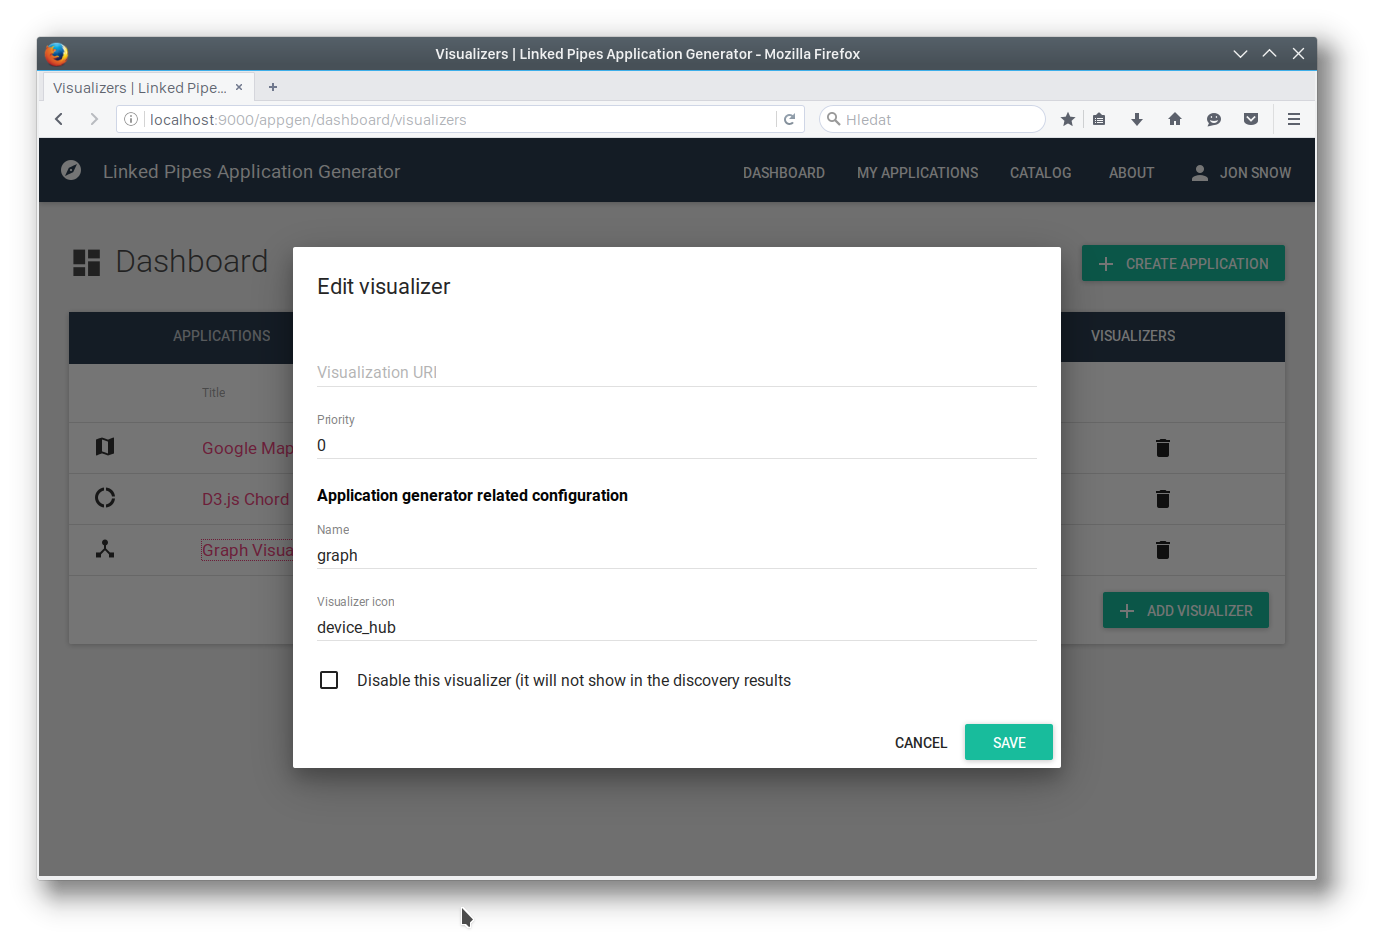
\includegraphics[width=140mm]{img/05_edit_visualizer.png}
	\caption{Configuration dialog window of a \emph{visualizer}.} 
	\label{fig:edit-visualizer}
\end{figure}
This was the last mandatory step. At this moment, the \emph{visualizer} (even though it does not do anything) should be working, i.e., it should be possible to create a new application using this \emph{visualizer} from a data set containing graph data.

\subsection{Scala backend}

Surprisingly enough, we did not have to touch the Scala backend to register our new \emph{visualizer}. Technically speaking, it is really not necessary but only until the very moment when we need the \emph{visualizer} to actually \textit{do something useful}. That typically involves fetching and extracting the RDF data produced by the \emph{pipeline}. For that we do need the backend.

In this subsection, we will simply prepare the controller that will be handling our client requests.

\begin{verbatim}
package controllers.appgen.api.visualizers
import scaldi.Injector

class GraphVisualizerApiController(implicit inj: Injector) extends VisualizerApiController { }
\end{verbatim}

The package information clearly says where this class should belong. The \texttt{VisualizerApiController} will provide us with some utilities that will come handy later.

\subsection{Extracting RDF data from the pipeline evaluation}

We said that our \emph{visualizer} would show the number of vertices and edges in the graph. For us that means that we need to access the RDF data produced by the \emph{pipeline}, extract this information from it, send it to the client and then display it on the screen. We start with accessing the RDF data.

Since it is RDF data, we will use SPARQL queries to fetch the information we need. 

\begin{verbatim}
package model.rdf.sparql.rgml.query
import model.rdf.sparql.query.SparqlQuery

class GraphQuery extends SparqlQuery {

  def get: String =
    """
      | PREFIX rdf: <http://www.w3.org/1999/02/22-rdf-syntax-ns#>
      | PREFIX rgml: <http://purl.org/puninj/2001/05/rgml-schema#>
      |
      | SELECT ?directed ?nodeCount ?edgeCount WHERE {
      |   ?graph
      |     rdf:type rgml:Graph ;
      |     rgml:directed ?directed .
      |
      |   { SELECT (COUNT(*) AS ?nodeCount) WHERE { ?edge rdf:type rgml:Node . } }
      |   { SELECT (COUNT(*) AS ?edgeCount) WHERE { ?edge rdf:type rgml:Edge . } }
      | }
      | LIMIT 1
    """
      .stripMargin
}
\end{verbatim}

This is the recommended way of representing SPARQL queries in our Scala code. As you can see, the query counts all the edges and vertices (which are called \emph{nodes} in the RGML vocabulary) and also fetches the information about whether the graph is directed or not.

The result of this query will be represented using a simple Scala case class. For simplicity, we just call it \texttt{Graph}.

\begin{verbatim}
package model.rdf.sparql.rgml

case class Graph(directed: Boolean, nodeCount: Int, edgeCount: Int)
\end{verbatim}

Now we need a tool that will convert the fetched RDF data into this case class. Such a tool is called an \emph{extractor}.

\begin{verbatim}
package model.rdf.sparql.rgml.extractor

import model.rdf.extractor.QueryExecutionResultExtractor
import model.rdf.sparql.rgml.Graph
import model.rdf.sparql.rgml.query.GraphQuery
import org.apache.jena.query.QueryExecution


class GraphExtractor extends QueryExecutionResultExtractor[GraphQuery, Graph] {

  def extract(input: QueryExecution): Option[Graph] = {

    try {
      val resultSet = input.execSelect()

      if (!resultSet.hasNext) return None

      val solution = resultSet.nextSolution()
      Some(Graph(
        solution.getLiteral("directed").getBoolean,
        solution.getLiteral("nodeCount").getInt,
        solution.getLiteral("edgeCount").getInt))
    } catch {
      case e: org.apache.jena.sparql.engine.http.QueryExceptionHTTP => {
        None
      }
    }
  }
}
\end{verbatim}

Apache Jena \footnote{https://jena.apache.org/} framework is used internally to work with RDF data. Our SPARQL query is a SELECT query which means that the results will be in a form of tabular data (i.e., a set of rows where each row contains the same columns). We assume that the data set contains only one graph, so we take the first row (if available) and convert it to the \texttt{Graph} case class.

Finally, we need something that will execute the query and apply the extractor on the results.

\begin{verbatim}
package model.rdf.sparql.rgml
//  ...imports

class RgmlService(implicit val inj: Injector) extends RgmlService with Injectable {
  var sparqlEndpointService = inject[SparqlEndpointService]

  def graph(evaluation: PipelineEvaluation)(implicit session: Session): Option[Graph] = {
    sparqlEndpointService.getResult(
      evaluationToSparqlEndpoint(evaluation),
      new GraphQuery(),
      new GraphExtractor())
  }
\end{verbatim}

As you can see, we defined \texttt{RgmlService} with the \texttt{graph} method. The \emph{pipeline evaluation} does not directly contain the data but rather points where the data are (i.e., it specifies the SPARQL endpoint and concrete named graphs with the data). We use \texttt{SparqlEndpointService} to access it and extract our graph from it. The function \texttt{evaluationToSparqlEndpoint} is just an utility that we omitted to keep the code short. % TODO: add it to a trait

You might have noticed that we put all the files in the same package \texttt{model.rdf.sparql.rgml}. What we are doing is that we are adding support for RGML vocabulary to the LinkedPipes Visualization code base in a way that anyone can use it for their \emph{visualizers}, i.e., it is \emph{visualizer} independent.

For the \texttt{RgmlService} to work properly, it has to be registered to the Dependency Injection container in \texttt{model.rdf.RdfModule}.

Let us now move from the \emph{Model} layer to the \emph{Controller} layer. We will extend the controller we defined earlier with an action that will use this service to fetch graph and send it to the client serialized to JSON.

\begin{verbatim}
class GraphVisualizerApiController(implicit inj: Injector) extends VisualizerApiController {
  val rgmlService = inject[RgmlService]

  def getGraph(id: Long) = RestAsyncAction[EmptyRequest] { implicit request => json =>
    withEvaluation(ApplicationId(id)) { evaluation =>
      val graph = rgmlService.graph(evaluation)
      Future(Ok(SuccessResponse(data = Seq("graph" -> graph))))
    }
  }
}
\end{verbatim}

The \texttt{getGraph} action is mapped to a URL with a single parameter \texttt{id} (the URL mappings are defined in the file \texttt{src/conf/routes}, relative to the code base root). The \texttt{id} is an application ID. We use the \texttt{withEvaluation()} helper to load the appropriate \emph{pipeline evaluation}, then we fetch the graph using our \texttt{RgmlService} and send it to the client in a \texttt{SuccessReponse}. The API is designed to support \texttt{Futures} in case the requests are expected to be computationally heavy and need t.jso be performed asynchronously. This is not our case but we need to follow the API. That is why the response is wrapped by the \texttt{Future} call.

In order for the \texttt{Graph} case class to be automatically converted to JSON, we need to define an \emph{implicit converter}. We can do it by adding following lines to \texttt{controllers.api.JsonImplicits} and import it to the controller:

\begin{verbatim}
implicit val graphWrites = Json.writes[Graph]
\end{verbatim}

\subsection{Making asynchronous requests from the client}

Everything is prepared on the server-side. Now comes the client. When the application loads, we will make an synchronous HTTP request to fetch the graph information. Once we receive it, we store it in the \emph{state} and show it on the screen.

We start by creating a JavaScript counterpart for the Scala \texttt{Graph} case class. Note that once again, all paths are relative to the \emph{visualizer} module.

\begin{verbatim}
// models.js

import { Record } from 'immutable';

export const Graph = Record({
  directed: false,
  nodeCount: 0,
  edgeCount: 0
});
\end{verbatim}

We create a simple explicit wrapper for the asynchronous HTTP request.

\begin{verbatim}
// api.js

import rest from '../../../misc/rest'

export async function getGraph(applicationId) {
  const result = await rest('graphVisualizer/getGraph/' + applicationId, {});
  return result.data.graph;
}
\end{verbatim}

The keywords \texttt{async/await} are just syntactical sugar around \texttt{Promises}. They allow us to write \emph{asynchronous} code in a \emph{synchronous} manner.

Now we will define a new \emph{duck} that will handle and provide API for fetching the graph information, storing it in the \emph{state} and selecting it from the \emph{state}.

\subsection{Adding editable resource label}

% TODO: Give credit to the LDVM guys

\section{Advanced framework features}

\subsection{Saving and loading application configuration}

\subsection{Multiple language support}

\subsection{Label dereferencing}

\subsection{Custom label editor}

\subsection{Embedding applications}

\subsection{Miscellaneous}

\section{Design choices regarding the framework}

\subsection{Integration of new visualizers}

% Why the URL contains visualizer name

% Explain that this kind of integration is incredibly flexible (first on the standalone/embed level, then in general, AngularJS, jQuery) 
% Completely free to do anything inside the components

